\documentclass[a4paper]{article}
\usepackage[fleqn]{amsmath}
\usepackage{kpfonts}
\usepackage[section]{placeins}
\usepackage{epsfig}
\usepackage{secdot}
\usepackage{graphicx}
\usepackage{overpic}
\usepackage{amsfonts}
\usepackage{setspace}
\usepackage{verbatim}
\usepackage{secdot}
\usepackage{ctable}
\usepackage{amsmath}
\usepackage[all]{xy}
\usepackage[square,sort,comma,numbers]{natbib}
\usepackage{amsbsy}
\graphicspath{ {images/} }
\usepackage{wrapfig}
\usepackage{subfigure}
\usepackage{fullpage} % correct the margins
\usepackage[section]{placeins}
\usepackage{float}
\usepackage{amssymb}
\usepackage{algorithm}
\usepackage{algpseudocode}
\usepackage{enumerate}
%\usepackage{mathptmx}
\usepackage{algorithm,algorithmicx,algpseudocode}
\usepackage{mathtools}
\usepackage{dsfont}





\begin{document}
\title{Exploring hidden graph structures in flat dataset, and KiNN graph based model}
\author{joseph keshet}
\maketitle
\tableofcontents
\pagebreak
\abstract{
We live in a networked world  pages and people, web links and friendships are easily modeled as nodes and edges, combined into a graph structure and analyzed using techniques from graph theory and social network analysis(\emph{SNA}).  
While social ties are clear (you are either a friend or not), It isn't the case in many non social datasets. For example, whether ties exist between one movie record to another, and if a connection exists, what is the nature of the connection.
Those form two different data, source, a tabular flat dataset and graph structured dataset, each with it's own analysis techniques.
In this paper we will  like to the close the gap between those seemingly different approaches to explore hidden graph structures from flat out data, form a graph model which is both descriptive and predictive and test it against other known regression models, various simulated datasets  and real world movie revenues dataset.
}

\iffalse
like centrality measures (as the very known "PageRank"),clustering coefficient  ,diameter of the graph are just some examples.
As such , It is can  be analyzed using graph theory and social network analysis techniques 
\fi
\section{Motivation}
In a world connected with by global network,social networks play major role society and business.
where ,web pages are connected through hyperlinks, \emph{Facebook} is a network of social connections, \emph{LinkedIn}  promotes professional ties and so forth.\\
As it's name suggests, social data is often modeled in a network graph structure.
In social networks models, friendship is modeled as a binary relation, am I your friend {true/1}or not {false/0} as an edge between 2 nodes /people in a social graph.(Figure 1(a)).
However, in many datasets containing many variables with various types , it is not clear what is the nature of edge/link.
For instance, how to we connect movies in a network structure?
Also graph based models are often used for clustering 
and as a descriptive rather than prediction(regression)
Many regression models (as linear regression) view data as a collection of variables/columns in a flat table structure, with some assumptions of the nature of the connection between predictor and outcome variables.
\begin{figure}[H]
\centering

\subfigure[facebook graph representation]{
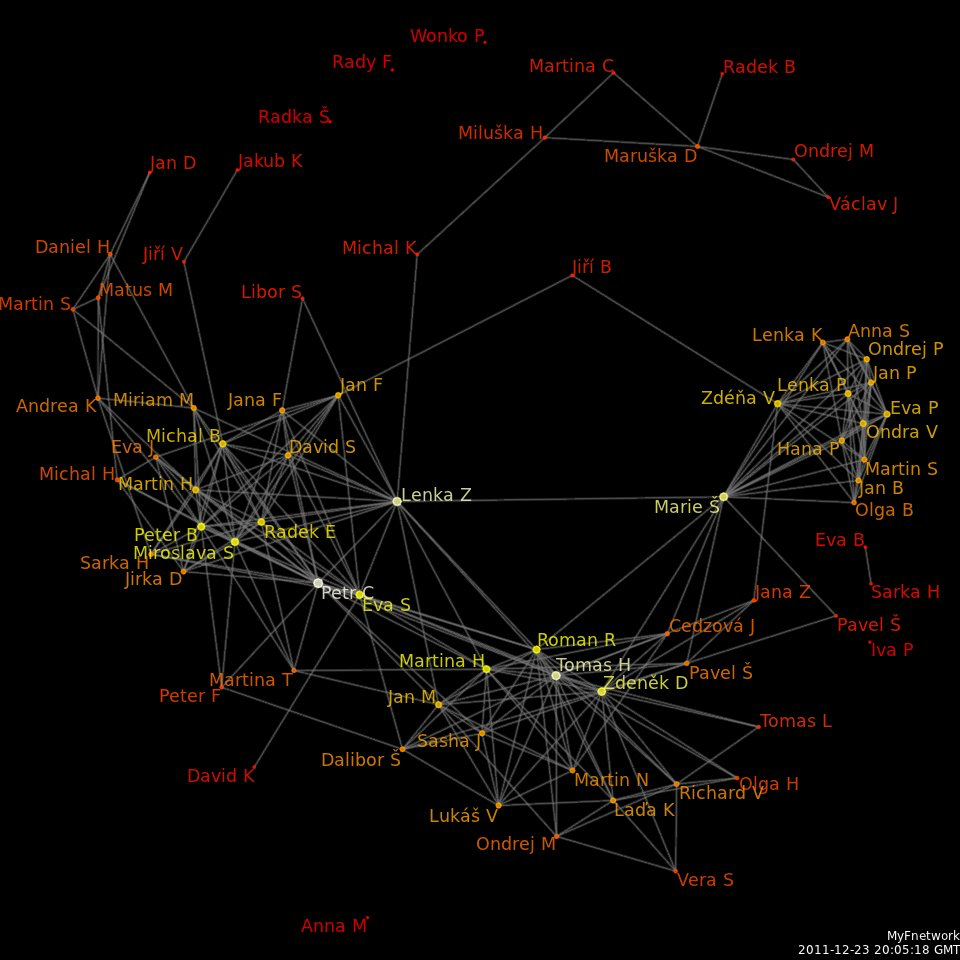
\includegraphics[width=0.4\textwidth,,height=4cm]{facebook}
 \label{fig:subfig1}	
 }
 \centering
\subfigure[business data in tabular form]{
    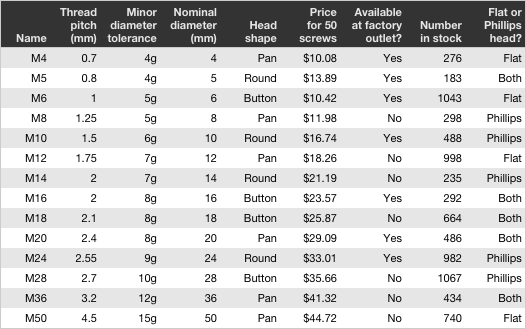
\includegraphics[width=0.4\textwidth]{data-table}
    \label{fig:subfig2}
}

\caption[Optional caption for list of figures]{
Graph Vs Flat data.
}
\end{figure}
Our goal in this paper is to merge those two seemingly different approaches  to form new prediction and description model of the data, by finding hidden networks in dataset.
Using this approach we can import methods and techniques from \emph{SNA}(and vise versa),gain intuition and insights about the data by representing multi-variable/dimension data in graph structure.
In this model we will also make\emph{ no assumptions} about nature of the connection between regressors and outcome variable, may not be known or exist in analytic form but rather may change from point to point.
Using this model can be used as standalone prediction model or by incorporating graph model predictions as a latent data variable in known predictive models expressing additional graph information predictor variable. 

\subsection{background}
Several approaches were used to incorporate network structure techniques in analyzing  data sets. \\
In \textbf {Recommender Systems with Social Regularization}[1] \\
describes a  recommender framework, Two given matrices are used, Users Movie Ratings in scale 1-5 and social matrix where edge  i $\rightarrow$ j indicated that user i trusts user(friend) j.  Here Known social ties  are  used as friend movie preferences  are added as a regularization term to the minimization target function, counter balancing collaborative rating term. Similarity between users is defined using PCC("pearson" correlation coefficient) to weight each friend contribution in the regularization term instead of simple average (in case friends have diverse taste).  This method does not however find hidden structure but rather uses already known friendship graph matrix. \\
\\
In \textbf{Determining Patient Similarity in Medical Social Networks}[2], Similarity using user content is done by weighted sum of the differences in each variable.
The weight of each difference is determined differently according to the type of the variable. In case of discrete data, logistic regression is used where the probability of each variable 
given data provides its weight to similarity  function.In case of continues variable, 
proportional hazard regression (Cox regression) is used. 
While finding the similarity measure and handling both categorical and continuous variables,
\emph{Social graph data is ignored due to the hypothesis that content based similarities is superior to social in medical systems}  \\
\textbf{SimRank: A Measure of Structural-Context Similarity }[3]\\
Analogies to “PageRank”  similarity is defined by using bipartite graph of categorical variables recursively. 
objects are similar as their features.
features are similar as the objects which contains them.
• People are similar if they purchase similar items. 
• Items are similar if they are purchased by similar people. 
and  iterating between object similarity and features similarity
till convergence is achieved.
running page rank on similarity matrix gives the final similarity. \emph{While tackling  similarity in  graph structure manner, it handles only categorical variables ignoring continuous variables measures.}\\
\\
\textbf{A Graph-based Recommender System for Digital Library} [4] Using a graph-based recommender combines the content-based and  collaborative approaches into hybrid  based system .
The model is based on to layers book layer and user layer(inner layer links) and the connection between the two layers(inter layers links).
In the content-based book layer, each node represents a book, while each link between any two books represents the content similarity between them. Each node in the customer layer represents a customer, and links between customer nodes are the demographic similarity between the two customers. Besides the inner layer links, inter-layer links are also available in the graph model. These links are based on the purchase histories of all customers, wherein a purchase is represented by a link between a node in the book layer and a node in the customer (directed from user to book purchase) layer thus combining book content based layer graph to user based layer into a hybrid recommender graph based system In a book graph layer a content similarity measure is applied to each pair of books (edge) while in the customer layer demographic based similarity is computed. 
The inter layer links between book layer and customer layer is simply derived from purchase history. Each link in the graph has a weight between 0 and 1.
Finally association between  book B and customer C
 is computed as a sum of all paths measure between B and C when path measure is a multiple of similarities along the path.
The high-degree association recommendation can be treated as a concept retrieval task. 
While this method creates a graph like structure between layers , each node whithin  a layer(iiner link  is connected resulting a clique sized layer.
Also content-based approach performed better over the collaborative and hybrid approaches,
explained by the hypothesis subjects tended to relay heavily on the book content information.
\\ 
\\ 
\textbf{ Mining Hidden Community in Heterogeneous Social Networks}[5]
Most of the existing algorithms on social network analysis assume that there is only one single social network, representing a relatively homogeneous relationship (such as Web page linkage). In real social networks, there always exist various kinds of relations. Each relation can be treated as a relation network.
Given various relations of objects, a linear combination of relations is found which can best reveal the intrinsic relationship between the objects with respect to the user's query.
The algorithm tries to  find  combined relation which makes the relationship between the
 intra-community examples as tight as possible and at the same time the relationship between the inter-community examples as loose as possible.
inter relation and intra relation are represented by matrices and linear combination of matrices must match the inter relations matrix using constrained linear regression (\emph{"Ridge Regression"}).
when the examples provided by the user belong to only one community, a "\emph{minimal cut }  approach is done 
when we minimize the the minimal cut of a linear combination of the intra relations graphs.
with respect to coefficients of community matrix/graph.
This approach  has the disadvantage that single community can be found to often in large datasets.
The algorithm also creates  matrix for each community relation and one for intra relation, a solution which might be memory exhaustive. 
 \\
\\
\textbf{Modeling Social Strength in Social Media Community via Kernel-based Learning}[6]
One of the key issues in social strength modeling (SSM) is how to effectively explore the heterogeneous data and how to optimally combine them to measure the social strength.
In order to deal with heterogeneous data, each type of data(modality) (such as picture,tags etc) is given a similarity function (kernel)of its own(up to a total of 7 different kernels).
Combining these modalities  is done by in linear combination of multiple kernels to fuse all modalities into single measure function.
Kernel alignment method is then used to measure the quality of kernel K with respect to the target matrix Y,  which encodes the \emph{existing known} relationship among users (through explicit friend lists), and evaluating the weights of the kernels in the linear combination.
Once a (single)similarity measure is found  a discriminative model is used to estimate the social strength between two users and indicate whether there is a connection between two users by logistic normal model.
although MKL(multiple kernel learning) outperformed single kernel and uniform weights for each kernel,
/emph{The most crucial element of a kernel method  is choosing the right kernel which is not a trivial task
It uses a known links between users as a target function which may not be available when links are hidden and not available for training}.

In \textbf{Ordering Points To Identify the Clustering Structure}[11] the product of the clustering algorithm yields an ordering
which can interpreted as a structure of the cluster.
however in as kNN depends upon minPoints parameter
per cluster and does not concern with prection 
and amount of edges needed for that.optics X reachability graph may be highly connected  however points in y axis
might lay on a perfect line with no need for more that one edge
or two for prediction)
 
however, edges 

\pagebreak

\section{Existing Prediction Models}
In this section we regression models which will be used to benchmark our graph model.


\subsection{Linear Regression}
Given a data set $ (Y_i,\, X_{i1}, \ldots, X_{ip}),\quad i=1,..,n $ of n statistical units, 
a linear regression model assumes that the relationship between the dependent variable $Y_i$ and the p-vector of regressors $X_i$ is linear. 
\\This relationship is modeled through a disturbance term or error variable$ ε_i $— an unobserved random variable that adds noise to the linear relationship between the dependent variable and regressors. Thus the model takes the form:\\
$ Y_i = \beta_1 X_{i1} + \cdots + \beta_p X_{ip} + \varepsilon_i
 = X^{\rm T}_i\beta + \varepsilon_i, \quad i = 1, \ldots, n.$\\
where T denotes the transpose, so that $X_i^T\beta$ is the inner product between vectors
    $X_i $and $\beta$.\\
The regression coefficients $\beta_0, \beta_1,...,\beta_p $ are unknown, and are be estimated using a least squares approach. Given  estimates $\hat\beta_0, \hat\beta_1,...,\hat{\beta_p} $  we can make predictions using the formula 
$\hat{Y}= \hat\beta_0x_0+\hat\beta_1x_1+...+\hat{\beta_p}x_p $.


\subsection{k-NN Regression}
K-nearest neighbors regression (k-NN regression) 
is a non-parametric method which given a value for K and a prediction point $x_0$, k-NN
regression first identifies the K training observations that are closest to
$x_0$, represented by $N_0$. It then estimates $f(x_0)$ using the average of all the
training responses in $N_0$.\\

$\hat f(x_0) = \dfrac{1}{K} \sum\limits_{x_i \in N_0} y_i.$\\
 In general, the optimal value
for K will depend on the bias-variance tradeoff. \\
A small value for K provides the most flexible fit, which will have low bias but high variance. This variance is due to the fact that the prediction in a given region is entirely dependent on just one observation.
In contrast, larger values of K provide a smoother and less variable fit. The
prediction in a region is an average of several points, and so changing one observation has a smaller effect. However, the smoothing may cause bias by masking some of the structure in $f(X)$.

\subsection{Classification and Regression Tree (CART)}
Despite the name, regression trees do not use linear regression, rather, they make predictions based on the average value of examples that reach a leaf.
Trees for numeric prediction are built in much the same way as they are for classification. Beginning at the root node, the data are partitioned using a divide-and-conquer strategy according to the feature that will result in the greatest increase in homogeneity in the outcome after a split is performed.  For numeric decision trees, homogeneity can be measured by statistics such as variance, standard deviation, or absolute deviation from the mean. Depending on the tree growing algorithm used, the homogeneity measure may vary, but the principles are basically the same.
A common splitting criterion is called the standard deviation reduction (SDR) which is defined in the formula\\
$SDR = sd(T) - \sum\limits_{i}\dfrac{|T_i|}{|T|} sd(T)$
In this formula, the $sd(T)$ function refers to the standard deviation of the values in set $T$, while $T_1 , T_2 , … T_n$ are sets of values resulting from a split on a feature.\\ The $|T|$ term refers to the number of observations in set T. Essentially, the formula measures the reduction in standard deviation from the original value to the weighted standard deviation post-split.
The feature for which "SDR" is minimal(greatest reduction in sd) is picked
for splitting and the process continues recursively for the rest of the features.
\\
\\
*\emph{Those models will be used as benchmark for our model predictions in the experiments section.
linear regression as are representative of flat data parametric model,
regression tree creates both descriptive and predictive in non linear tree model, knn a non parametric based upon similarity with fixed K neighbors.
}

\pagebreak
\section{KiNN Algorithm Description}
\subsection{Preliminary}
\subsubsection{Mixture Models}
A mixture model is a probabilistic model for representing the presence of subpopulations within an overall population, without requiring that an observed data set should identify the sub-population to which an individual observation belongs. (i.e sub populations are hidden)
Formally a mixture model corresponds to the mixture distribution that represents the probability distribution of observations in the overall population. However, while problems associated with "mixture distributions" relate to deriving the properties of the overall population from those of the sub-populations, "mixture models" are used to make statistical inferences about the properties of the sub-populations given only observations on the pooled population, without sub-population identity information.
\emph {General mixture model}
A typical finite-dimensional mixture model is a hierarchical model consisting of the following components:
N random variables corresponding to observations, each assumed to be distributed according to a mixture of K components, with each component belonging to the same parametric family of distributions (e.g., all Normal, all Zipfian, etc.)\\
 but with different parameters N corresponding random latent variables specifying the identity of the mixture component of each observation, each distributed according to a K-dimensional categorical distribution\\
A set of K mixture weights, each of which is a probability (a real number between 0 and 1 inclusive), all of which sum to 1
A set of K parameters, each specifying the parameter of the corresponding mixture component. In many cases, each "parameter" is actually a set of parameters. For example, observations distributed according to a mixture of one-dimensional Gaussian distributions will have a mean and variance for each component. Observations distributed according to a mixture of V-dimensional categorical distributions (e.g., when each observation is a word from a vocabulary of size V) will have a vector of V probabilities, collectively summing to 1.\\
In addition, in a Bayesian setting, the mixture weights and parameters will themselves be random variables, and prior distributions will be placed over the variables. In such a case, the weights are typically viewed as a K-dimensional random vector drawn from a Dirichlet distribution (the conjugate prior of the categorical distribution), and the parameters will be distributed according to their respective conjugate priors.


\subsubsection{Expectation Maximization}
The EM algorithm is used to find the maximum likelihood parameters of a statistical model in cases where the equations cannot be solved directly. Typically these models involve latent variables in addition to unknown parameters and known data observations. That is, either there are missing values among the data, or the model can be formulated more simply by assuming the existence of additional unobserved data points. For example, a mixture model can be described more simply by assuming that each observed data point has a corresponding unobserved data point, or latent variable, specifying the mixture component that each data point belongs to.
Expectation maximization (EM) is seemingly the most popular technique used to determine the parameters of a mixture with an a priori given number of components. This is a particular way of implementing maximum likelihood estimation for this problem. EM is of particular appeal for finite normal mixtures where closed-form expressions are possible such as in the following iterative algorithm by Dempster et al. (1977)[8]
\emph{The expectation step}
With initial guesses for the parameters of our mixture model, "partial membership" of each data point in each constituent distribution is computed by calculating expectation values for the membership variables of each data point. That is, for each data point $x_j$ and distribution $Y_i$, the membership value $y_i, j$ is:

$y_i,_j=\dfrac{f_Y(x_j;\theta_j)}{f_X(x_j)}$\\
The maximization step
With expectation values in hand for group membership, plug-in estimates are recomputed for the distribution parameters.
The mixing coefficients $a_i$ are the means of the membership values over the N data points.\\

$a_i=\dfrac{1}{N} \sum\limits_{j=1}^{N} y_i,_j$

The component model parameters $\theta_i$ are also calculated by expectation maximization using data points $x_j$ that have been weighted using the membership values. \\
For example, if $\theta$ is a mean $\mu$\\
  $ \mu_i=\dfrac{\sum\limits_{j}y_{i,j} x_j}{\sum\limits_j{y_{i,j}}}$

With new estimates for $a_i$ and the $\theta_i$'s, the expectation step is repeated to recompute new membership values. The entire procedure is repeated until model parameters converge.
\\
\subsubsection{Kernel Similarity}
kernel function is   \emph{generalization} of the inner product of the form
$K (x_i , x_{i'} )$,
where K is some function that we will refer to as a\emph{kernel} . A kernel is a function that quantifies the similarity of two observations. For instance, we
kernel
could simply take
$ K (x_i , x_{i'} )=\sum_{ j=1}^{p} x_{ij} , x_{i'j}$
this linear kernel essentially quantifies the similarity of a pair of observations using Pearson (standard) correlation. But one could instead choose another form For instance, instance of
$ K (x_i , x_{i'} )=(1+\sum_{ j=1}^{p} x_{ij} , x_{i'j})^d$.\\
This is known as a polynomial kernel of degree d, where d is a positive integer. Using such a kernel with d > 1, instead of the standard linear kernel and  leads to a much more flexible decision boundary. It essentially amounts to fitting a support vector classifier in a higher-dimensional space involving polynomials of degree d, rather than in the original feature space. 
Another popular choice is the radial kernel, which takes the form
$ K (x_i , x_{i'} )=exp(\sum_{ j=1}^{p} x_{ij} , x_{i'j})^2$.\\
kernels offer computational benefit since kernel function can be 
computed in original feature space without the need to tp map
and compute in higher dimensions spaces.(Kernel )
(In such as the radial kernel  the feature space is implicit and infinite-dimensional, so we could never do the computations there anyway)
\\
\subsubsection{Social Network Analysis(SNA)}
Social network analysis (SNA) is the use of network theory to analyze social networks. Social network analysis views social relationships in terms of network theory, consisting of nodes, representing individual actors within the network, and ties which represent relationships between the individuals, such as friendship, kinship, organizations and sexual relationships.[1][2] These networks are often depicted in a social network diagram, where nodes are represented as points and ties are represented as lines.
Social network analysis is used extensively in a wide range of applications and disciplines. Some common network analysis applications include data aggregation and mining, network propagation modeling, network modeling and sampling, user attribute and behavior analysis, community-maintained resource support, location-based interaction analysis, social sharing and filtering, recommender systems development, and link prediction and entity resolution.[35] In the private sector, businesses use social network analysis to support activities such as customer interaction and analysis, marketing, and business intelligence needs. Some public sector uses include development of leader engagement strategies, analysis of individual and group engagement and media use, and community-based problem solving.



Our model tries to capture hidden patterns in order to use this hidden information to for prediction.
It does it two consecutive steps which defines two layer of similarity:


.
 
 \pagebreak
 
\paragraph{General Framework}\hspace{0pt}\\
This section describes the  algorithm for prediction model in  $\mathbb{R}$.\\
\emph{Let:}	 \\
\begin{equation}
X=\{x_i\in \mathbb{R} \} \quad
Y=\{y_i\in \mathbb{R} \} \quad
f:X\rightarrow Y
\end{equation}
%\end{flalign*}
Be a regressor group,   its outcome group, and a mapping  accordingly
\emph{Such that:} \\ 
\begin{equation}
f(x_i)=y_i,\quad\forall  i=1\dots n .\\
\end{equation}
We make is no prior assumption on the nature of the connection between a predictor and outcome variables.It may be linear,non linear, exponential, or have no known analytic form.
We'll model the data as a graph, where each $x\in X$ form a node,which is connected to other close nodes(neighbors).
An estimator $\hat{y}$ is then calculated by linking predictor x (with unknown y) to 
a prediction set,  which is made out of most similar node ,$x_s$   and  $x_s$ neighbors in a graph. Then, The outcome variables of the prediction set in the graph are extracted and those values are used to prediction(for instance by averaging).
Graph structure will help us to capture different shapes of the data and form a descriptive model, and will be able to find a  prediction set, whose  size may vary from node per node.
\begin{figure}[ht]
\centering
\subfigure{
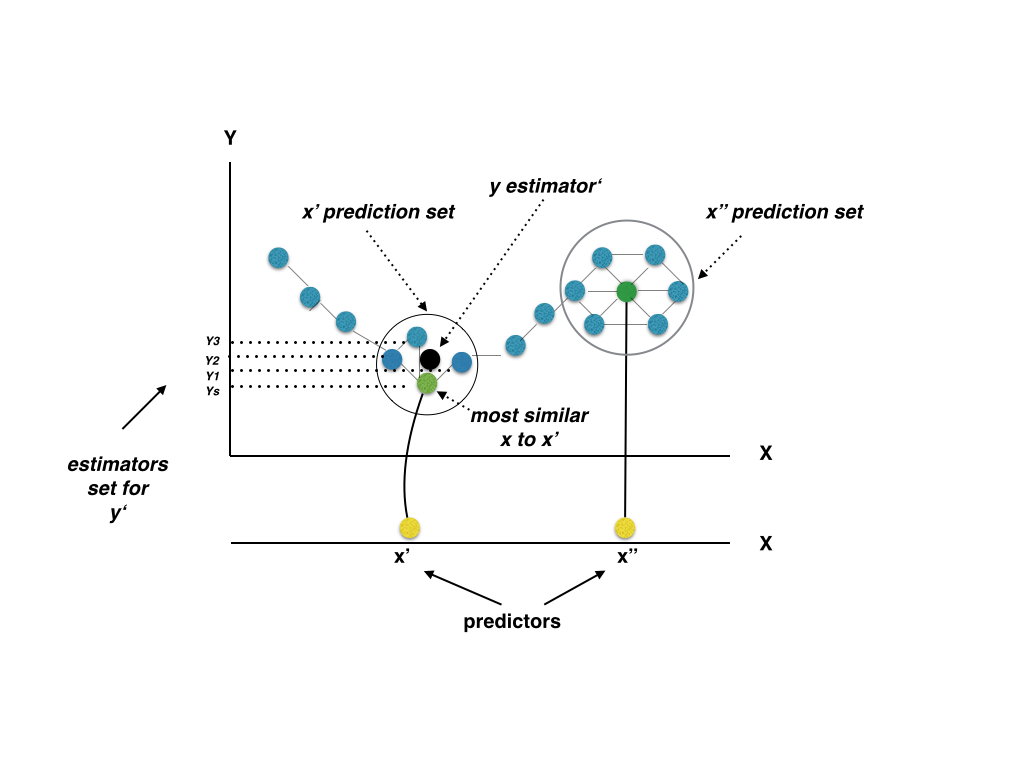
\includegraphics[width=0.6\textwidth,height=6cm]{drawings_010.png}    \label{fig:x-y}	}
\caption[Optional caption for list of figures]{making prediction by linking a predictor x to a group of connected nodes in the prediction graph. }
\label{fig:subfigureExample}
\end{figure}
Construction the  graph framework is comprised mainly out of 4 parts:
Modeling data in 1-d and 2-d domains, choosing similarity function and edge selection process.
The Final model is a set of prediction graphs,1-d and 2-d model parameters and the similarity function.
$(\{G{_i}\},M_{1d},M_{2d},Sim)$

\iffalse.
\begin{figure}[ht]
\centering
\subfigure{
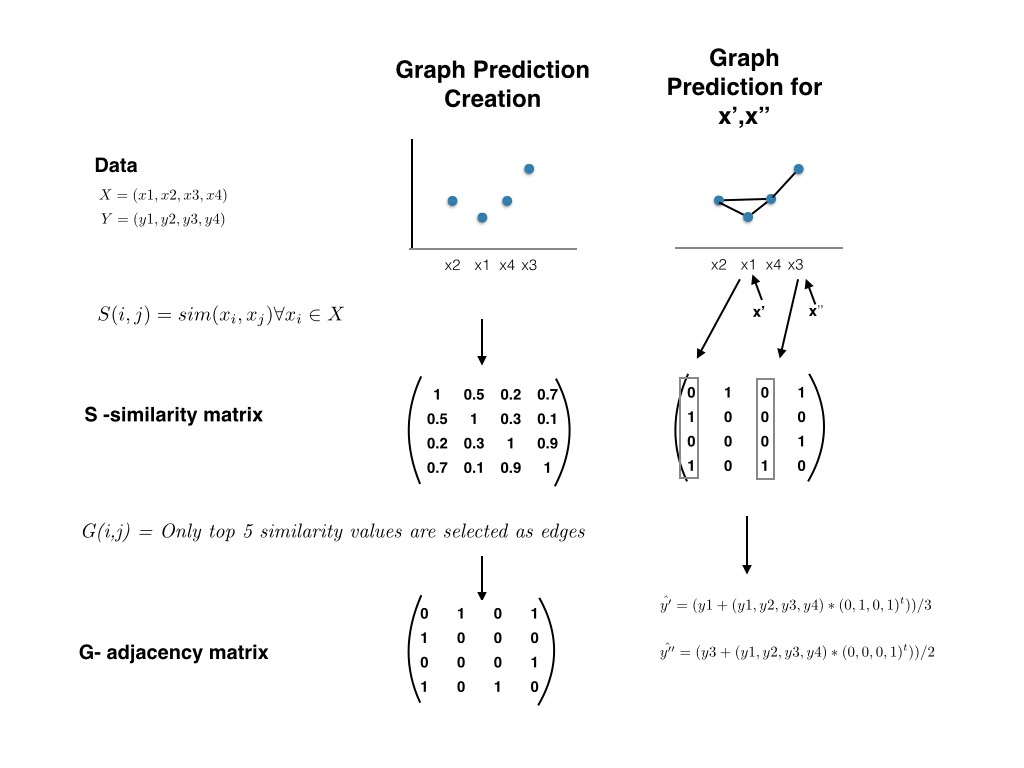
\includegraphics[width=0.6\textwidth,height=6cm]{drawings_009.png}    \label{fig:x-y}	}
\caption[Optional caption for list of figures]{making prediction by linking a predictor x to a group of connected nodes in the prediction graph. }
\label{fig:subfigureExample}
\end{figure}
\fi
\subsection{Similarity Groups in X }
Since We do not assume any prior relation between X and Y, 
our first link to  the data and in prediction process is through X predictors set.\\
A dataset can be similarity homogeneous (single similarity group), or comprised out of several similarity groups which represent different phenomenas/patterns in the dataset .
\paragraph{Modeling the data in 1-D X Domain}\hspace{0pt}\\
We'll model regressors group X as of disjoint \emph{d} similarity groups, using a similarity function for mapping:
\begin{equation}
M_{1D} :X   \rightarrow {\lbrace X_i, i=1\dots d \rbrace}
\end{equation}
\begin{equation}
\bigcup\limits_{i=1}^{d}X_i = X\quad and \quad\bigcap\limits_{i=1}^{d}X_i=\varnothing, \quad  \forall i\dots d.
\end{equation}
Partition of the predictors set X into similarity groups has two purposes:
\begin{itemize}
\item Allowing different similarity measures within each similarity group. Those measures can be different metrics parameters , different features ,or an entirely different similarity functions for each group.
\item
This reason relates to edge selection part which is a later part of the algorithm. In that section, we intend allocate \textbf {\emph {limited amount of edges}} to the prediction graph based upon similarity values. A group with high similarity among it's members, might dominate other groups during edge selection phase and as a consequence, take most of the edges in the prediction graph living very sparse graph regions and many isolated vertices.
\end{itemize}
\iffalse
Techniques like \emph{Expectation-Maximization} can be used create a the density based model $M_{1D}_{density}$  find missing distribution parameters $\gamma = \{w_i, \mu_i, \Sigma_i\}$ with additional latent variable $z\in \lbrace 1\dots d \rbrace$ which determines which density group associated with each value $x_i\in X$ in the dataset,\\
$z=i\rightarrow w_i=1\ and\ w_j=0,\quad \forall j\neq i,\ i ,j\in \{1\dots d\}$.\\
allowing for even overlapping distributions to be distinguished from each other.\\
* Dominating similarity group will be explained later in section TBD.\\
In order to find similarity, will first group values having sames features.
Using density based will enable us to combine both metric and
structure.
As two x values in X  might be in close proximity/localized but belong 
to different distributions/structure which might describe different 
phenomenas.
Having density groups will also help us computing suitable similarity measure for each of the similarity groups separately.each distribution depends on its parameters like Standard Deviation which reflects upon metric measure.
 as well as disallow one similarity group from dominance over the others *.


\fi
\paragraph{Example: Modeling Group Similarity As a Gaussian Mixture Model(GMM)}\hspace{0pt} \\
Given density similarity measure, we'll model the data as  a Gaussian Mixture Model.
\begin{equation}
 p(x|\gamma) =\sum\limits_{i=1}^{d} w_i * g(x\ |\ \mu_{i}  , \Sigma_{i})\quad
 \gamma = \{(w_i, \mu_i, \Sigma_i)\  i = 1, . . . , d\}\quad  \sum\limits_{i=1}^{d} w_i=1\\
\end{equation}
We'll  add an additional constraint $w_i\in \{0,1\}$, for separation of each point into non overlapping groups.\\
To do this will map each point x to  a distinct the similarity group  by highest posteriori probability for component i.
Techniques like \emph{Expectation-Maximization} can be used to find  distribution parameters $\gamma = \{w_i, \mu_i, \Sigma_i\}$ with additional latent variable $z\in \lbrace 1\dots d \rbrace$ which determines which density/similarity group i is associated with each value $x_i\in X$ in the dataset,
allowing for even overlapping distributions to be distinguished from each other.\\
\begin{equation}
 M_{1D}(x) = max\quad \{\  i \ \mid\ p(i\mid x,\gamma) > p(j\mid x,\gamma) ,\  \forall i\in \{1..d\} \ \}
\end{equation} 
\begin{figure}[ht]
\centering
\subfigure[x-y dataset points graph]{
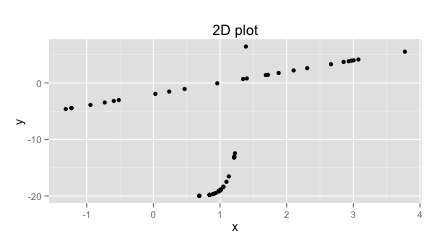
\includegraphics[width=0.4\textwidth]{img101}
   
    \label{fig:subfig1}	}
\subfigure[projection to x axis]{

    \includegraphics[width=0.4\textwidth]{img102}
    \label{fig:subfig2}
}
\subfigure[distribution similarity]{
    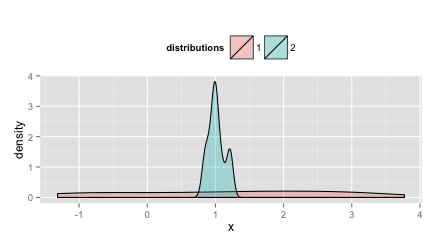
\includegraphics[width=0.4\textwidth]{img103}
    \label{fig:subfig3}
}
\subfigure[partition points in x axis]{
  %  \rule{4cm}{3cm}
  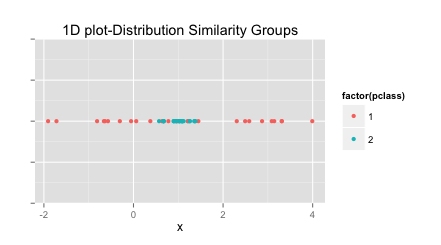
\includegraphics[width=0.4\textwidth]{img104}
    \label{fig:subfig4}
}
\subfigure[x-y with similarity group partition]{
  %  \rule{4cm}{3cm}
  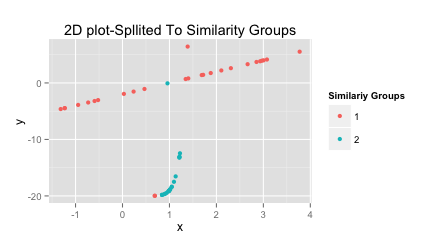
\includegraphics[width=0.4\textwidth]{img105}
    \label{fig:subfig5}
}
\caption[Optional caption for list of figures]
{\subref{fig:subfig1} 2-D points plot , clearly shoes two distinct patterns 
of linear and exponential functions.
\subref{fig:subfig2} Projection into X axis,results loss of dimensionality 
and no clear patterns.
 \subref{fig:subfig3}x axis distribution similarity
\subref{fig:subfig4} points in x axis are spllited according to their distribution patterns.
\subref{fig:subfig4} X-Y plot shoes  two distinct patterns based on 
data from only 1-D X axis and similarity distribution.}
\end{figure}
\pagebreak
\paragraph{Similarities Between Predictors Within Similarity Group }\hspace{0pt} \\
Our model is based upon similarity, the more similar values are, the 
greater likelihood of being connected in the prediction graph.
In order to do so, we need to choose a similarity function,
for calculating similarities between each pair .Those similarities form the similarity matrix which is the basis for the prediction graph adjacency matrix.\\
\emph{Let}
\begin{flalign*}
sim:X_i\times X_i \rightarrow \mathbb{R}_0^+
,\quad X_i=\{x_1,x_2,...,x_n\}
\end{flalign*}
be a similarity measure between 2 values in similarity group $X_i$.  \\A natural candidate for such a function can be \emph{Gaussian Kernel} similarity function  $sim(x_1,x_2)= e^{\|x_1-x_2\|}$.\\
Applying the similarity function for each pair $x_k,x_j\in X_i$ results in Similarity Matrix $S_i$
\begin{align*} 
s_{i,j} \equivֿ \{  sim(x_k, x_j)\quad  |\quad
x_i,x_j \in X_i,\quad 1 \leq k,j\leq nֿ\quad \}
\end{align*}
\begin{align*}  
  S_i \equiv
  \begin{pmatrix}
    s_{1,1}  & s_{1,2} & \cdots & s_{1,n}\\
    s_{2,1}  & s_{2,2} & \cdots & s_{2,n}\\
    \vdots & \vdots & \ddots &\vdots\\
    s_{n,1}  & s_{n,2} &\cdots & s_{n,n}\\
  \end{pmatrix}\quad
\end{align*}
This is a symmetric n $\times$ n matrix in which each row k, represents a vector of similarities between single member of the group $x_k$ and and all the group $X_i$ to which it belongs.\\
In order to avoid self similarity and overfitting, we'll zero the diagonal values by subtracting the identity matrix from the Similarity Matrix.
\begin{align*}
 S_i \leftarrow S_i - \mathds{1}=
  \begin{pmatrix}
    0  & s_{1,2} & \cdots & s_{1,n}\\
    s_{2,1}  & 0 & \cdots & s_{2,n}\\
    \vdots & \vdots & \ddots&\vdots\\
    s_{n,1}  & s_{n,2} &\cdots & 0\\
  \end{pmatrix} 
\end{align*}\\


\iffalse
A natural candidate for such a function is kernel similarity function
  \emph{Gaussian Kernel} $e^{\|x_1-x_2\|}$.\\
Within each similarity group $X_{i}$, calculate  similarity between each pair
in the group.
\fi
\subsection{Graph Adjacency Matrices From Similarity Matrices }
Once similarity Groups $X_i$ and similarity matrices $S_i$ are found, we'll construct a prediction graph $G_i(V_i,E_i)$ from the corresponding $X_i,S_i$.
Prediction graph is representation of the data set in a graph structure.
where each node represent x in the dataset, and edges connecting it to its neighbors groups  which  are most relevant x's for prediction.
This will be done in 3 stages:
\begin{enumerate}
\item Setting nodes set $V_i$
\item Calculating number of edges $|E_i|$.
\item Find edges group $E_i$ 
\end{enumerate}
\paragraph{Nodes group $V_i$ From $X_i$} 
Setting $V_i$ is trivial.\\
Each point in $X_i$ turns into a node in a graph vertices groups $V_i$.
\\Let  
\begin{align*}
X_i={x_1,x_2,..,x_n} \emph{\quad be a predcitor set}
\end{align*}
\begin{equation}
V_i\equiv X_i \ ,V_i=\{ v_k\mid v_k= x_k\quad  \forall x_k\in X_i\}\\
\end{equation}


\paragraph{Calculate Edges Cardinality $|E_i|$} 
Let  $K$ be edge density of a graph G(V,E) \\
\begin{equation}
K\equiv\dfrac{|E|}{|V|\times (|V|-1)}\\
\end{equation}
Hence edge cardinality:
\begin{equation}
\left \vert{E}\right\vert=K\times |V|\times (|V|-1)
\end{equation}
As $|V| $ is already known from previous stage ($|V|=|X|$)\\
we now need to calculate  edge density K.

\iffalse
As our prediction model is based upon similarity and similar values,
We'd  like to dilute the number of similarity values in matrices
for several reasons:

\begin{enumerate}

% style of 
\item  \emph{Computability} - Less numbers to crunch.
\item \emph{Accuracy}-
The noisier the graph the more values we need to smooth it and vice versa. 

\item \emph{Structurally}- Instead of clique like structure for each dataset,
(where every node is connected to each other), each  graph may have a different graph structure that could unveiled by removing unnecessary edges/connections.
\end{enumerate}
\fi

\paragraph{Noise as a measure of Edges Cardinality $|E_i|$.} 
In order to make prediction, we need to take only most similar values/neighbors in prediction graph into account during prediction process.
When no noise is present ,we'd like to allocate number edges a little as possible.
(less neighbors in the prediction graph)
When noise is significant, we'd like to smooth it by adding more values/edges.
As measure of noise, will take unexplained variable E(Var(Y$\mid$ X))\\

\begin{figure}[ht]
\centering
\subfigure[Y $\mid$ X shoes unexplained variability of response values in a noisy graph]{
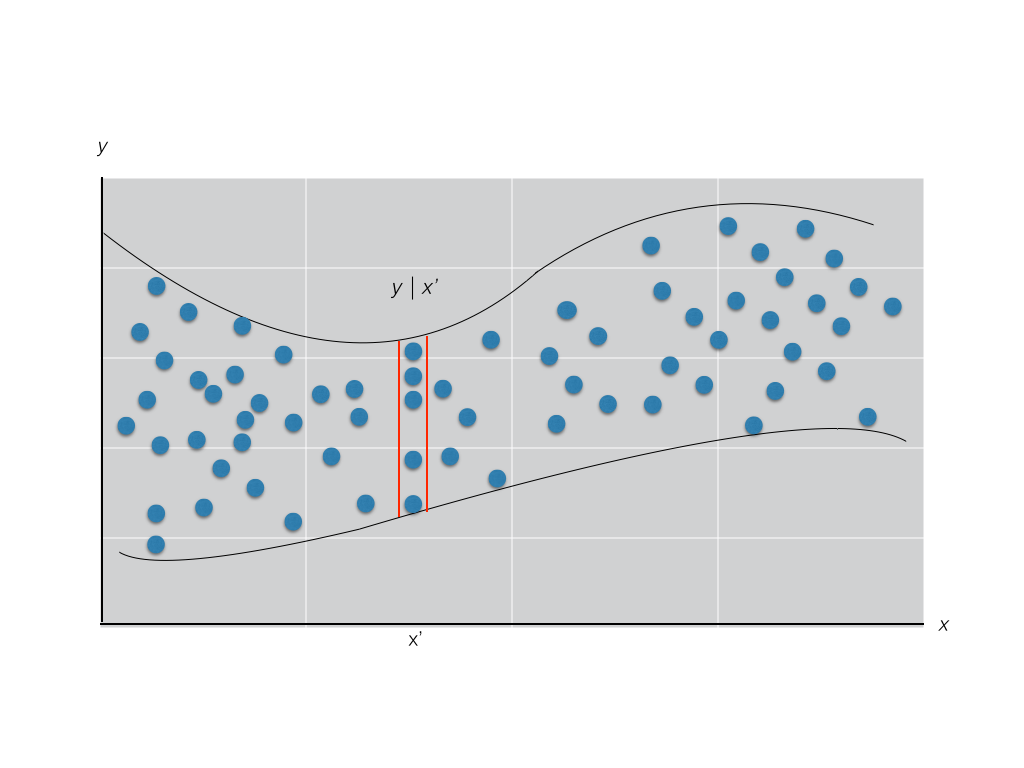
\includegraphics[width=0.4\textwidth,height=4cm]{drawings_004.png}   
 \label{fig:x-y}	}
\centering
\subfigure[Y $\mid$ X shoes low unexplained  variability in a low noise graph]{
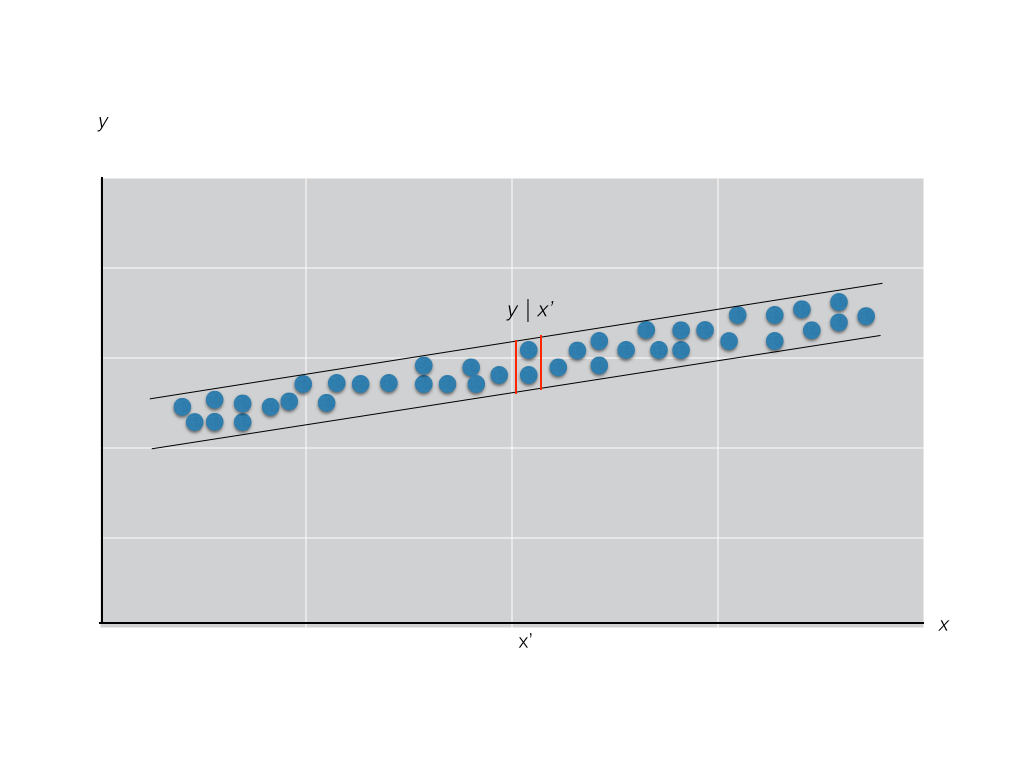
\includegraphics[width=0.4\textwidth,height=4cm]{drawings_005.png}   
 \label{fig:x-y}	}
\caption[Optional caption for list of figures]{Conditional Variance as a measure of noise
 }
\label{fig:subfigureExample}
\end{figure}

The law of total variance (also known as Eve's law)
\begin{equation}
Var(Y)=E(Var(Y\mid X)) +Var(E((Y\mid X)).
\end{equation}
Hence
\begin{equation}
E(Var(Y\mid X)) = Var(Y)-Var(E((Y\mid X)).
\end{equation}
In order to scale it to [0,1] interval, , we'll divide it by Var(Y) 
\begin{equation}
K  \propto \dfrac{E(Var(Y\mid X))}{Var(Y)} = 1 - \dfrac{Var(E(Y\mid X))}{Var(Y)}
\end{equation}
\paragraph{ Cardinality Of Edges  For A Linear Function} 
In case of \emph{Linear relationship} 
\begin{equation}
 E(Y \mid X) =aX+b
\end{equation}
\begin{equation}
\dfrac{ Var(E(Y \mid X))}{Var(Y)} =\dfrac{a^2\times Var(X)}{Var(Y)} =\dfrac{\dfrac{Cov(X,Y)^2\times Var(X)}{Var(X)^2}}{Var(Y)}=\dfrac{Cov(X,Y)^2}{Var(X)\times Var(Y)}=Corr(X,Y)^2
\end{equation}\\
Edge Density K
\begin{equation}
K \propto 1 -Corr(X,Y)^2=1-R^2
\end{equation}\\
And Edges Group Cardinality of a linear function:
\begin{equation}
\mid E_i \mid  \propto |X_i|\times (|X_i|-1) \times (1 -R^2)\propto  (|X_i|^2)\times (1 -R^2)
\end{equation}
Therefore linearity and low noise prefers low number of edges in the prediction graph.\\
More generally, when the conditional expectation E( Y $\mid$ X ) is a non-linear function of X,  K  be estimated as the R squared from a non-linear regression of Y on X, using data drawn from the joint distribution of (X,Y).
\begin{equation}
K \propto 1 - Corr(E(Y\mid X),Y)^2
\end{equation}
Now that we have edge density, we plug it into equation (10)
\begin{equation}
\mid E_i \mid  \equiv |X_i|\times (|X_i|-1) \times (1 - Corr(E(Y\mid X),Y)^2)
\end{equation}

\pagebreak
\paragraph{Calculating Edge Density Special Case - No Noise} \hspace{0pt}\\
In a case of  no or very little noise, for example, a function with high linearity  
\begin{equation}
Corr(x,y)^2 \longrightarrow 1,K \longrightarrow 0
\end{equation}
And as a consequence 
\begin{align*}
| E_i |\cong 0
\end{align*}
That is, no edges in a graph and no graph is formed.\\
To handle this case,lets look at a linear equation a strait line with no noise.\\
In drawing a prediction graph from points in a line (almost) every point is connected to only 2 points/friends in an undirected graph.
\begin{figure}[ht]
\centering
\subfigure{
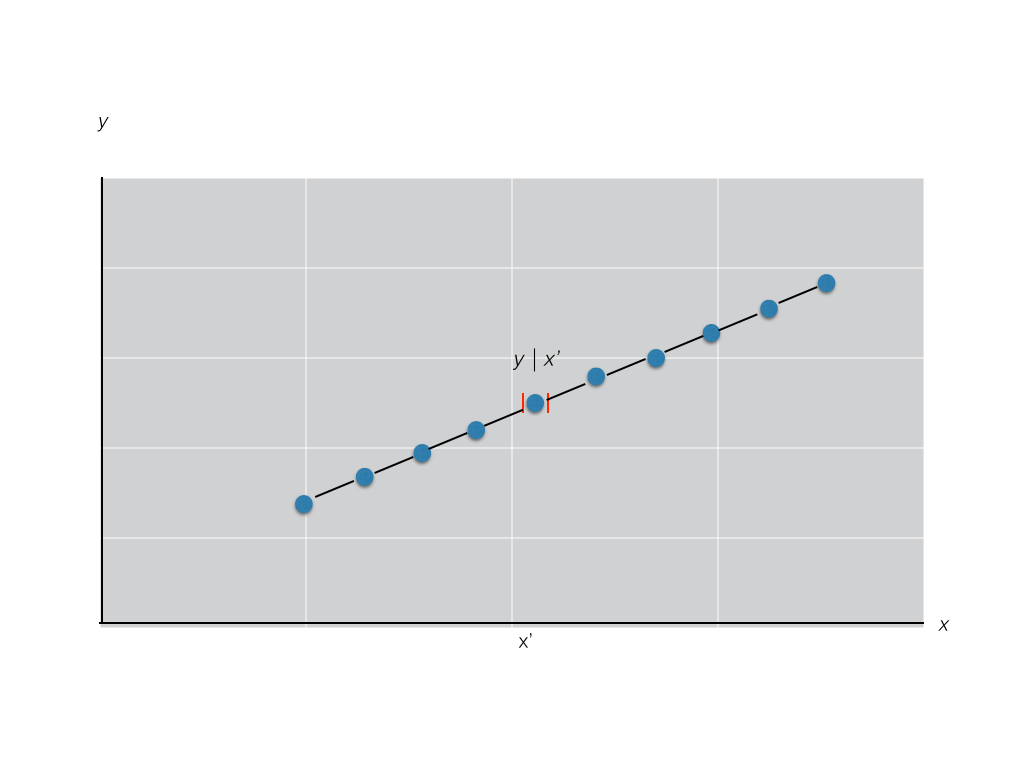
\includegraphics[width=0.4\textwidth,height=4cm]{drawings_006.png}   
 \label{fig:x-y}	}
\caption[Optional caption for list of figures]{Graph of Line,$Var(Y \mid X)=0$
 }
\label{fig:subfigureExample}
\end{figure}\\
So we the set lower bound value of edge density K to $\mid X_i\mid $\\
And the final formula for edges group cardinality:
\begin{equation}
\mid E_i \mid  \equiv max(\ \mid X_i\mid\  ,\  |X_i|\times (|X_i|-1) \times (1 -Corr(E(Y\mid X),Y)^2))
\end{equation}
\paragraph{Find Edges Group $E_i$ From Similarity Matrix $S_i$ And Edge Cardinality $\mid E_i \mid$}\hspace{0pt}\\
Once edge cardinality $\mid E_i \mid$ is found , the final step in constructing prediction graph is choosing the actual edges of the similarity prediction graph using the similarity matrix $S_i$ and $\mid E_i \mid$ .
Each value in similarity matrix $S_i$ can be viewed as an edge, connection measure between two nodes.
The higher the similarity - the stronger the connection or the higher probability that the two values are connected.Hence it is only natural to view similarity like so:\\
Let G(V,E) be a graph with known V, unknown E and Similarity Matrix S\\
\begin{align*} 
Probability( (v_j,v_k)\in G) \propto  Similarity(v_j,v_k) = S(i,j)=sim(x_i,x_j)
\end{align*}


Similarity Matrix resembles a dense correlation matrix and does not have a unique graph structure(probably a clique since every similarity matrix is most likely to have a positive number in each cell hence every node is connected  to each other )\\
Given that $\mid E \mid$ was already computed, we have several options to choose the edges for graph.
\begin{enumerate}
\item \textbf{ A Probabilistic Graph}\\
The approach of random graph was explored in  Erd\H{o}s-R\'enyi(ER) Model [9] .In ER  Model ,we set an edge between each pair of nodes with \emph{equal probability}, independently of the other edges. These models can be used in the probabilistic method to prove the existence of graphs satisfying various properties,with variable probability for each edge.
Here instead of equal probability for each edge,
We toss a biased coin based upon probability of an edge to appear in the graph.
As similarity is proportional to probability, higher similarity means a greater chance to be chosen, consequently the  probability for an edge to appear in a graph wold change from edge to edge.
In order to construct a random prediction graph, we  need to take into account several constraints:
\begin{itemize}
\item probability constraint $0\leq P(e)\leq 1,\quad \forall e\in E$
\item $\sum\limits_{e\in E} p(e)\times 1 = | E |$
\end{itemize}
So we construct probability matrix P By normalizing S to meet those two constraints.
a (very) naive normalization can be
\begin{align*}
P = S\times \dfrac{|E|}{\sum\limits_{i,j} s(i,j)}
\end{align*}
if similarity values turn out to be grater than one, we may need to re normalize
\begin{align*}
P \leftarrow	 P\times \dfrac{1}{\sum\limits_{i,j} p(i,j)}
\end{align*}
Another approach for the normalization problem is to do treat this as a  \emph{optimization problem}, with 
unknown probabilities p(i,j) and  the two constrains with a regularization term\begin{align*}
 \sum\limits_{i,j} \Vert s(i,j)-p(i,j)\Vert
\end{align*} as a penalty for digressing too much from similarity values.\\
\item  \textbf{A Deterministic Graph}\\
In this paper We'll opt for the deterministic method by choosing the Top $\mid E \mid$ similarity values from Similarity matrix as edges.
Once the values are chosen, an adjacency matrix is created
by setting  top $\mid E_i \mid$ values in similarity matrices $S_i$ to 1 and  the rest in $S_i$ to 0's.
\begin{equation}
Top(m,S) \equiv \{ \text{m highest values in group S} \}
\end{equation}
and edges are chosen for the adjacency matrix
 \begin{equation}     
   G(i, j)  = \begin{cases}
  1 & \quad \text{if $s_{i,j}\in Top(\mid E_i\mid,S_i)$ }\\
    0 & \quad \text{else }
\end{cases}
\label{eqn:simple_one} 
\end{equation}

resulting in adjacency matrices with binary values representing prediction subgraphs\\
\\
$\forall$  i $\in 1\dots d,\quad$
 $ G_i   =
  \begin{pmatrix}
    0  & 0 & \cdots & 1\\
    1  & 0 & \cdots & 0\\
    \vdots & \vdots & \ddots&\vdots\\
    1 & 0 &\cdots & 0\\
  \end{pmatrix}\\
$  

and 
\begin{equation}
E_i \equiv \lbrace \ (x_i,x_j) \quad \mid \quad		G_i(i,j) = 1 ,\   x_i,x_j \in X_i\  \}
\end{equation}


Thus we now have completed our prediction Graph $G_i(V_i,E_i)$.\\


\end{enumerate}

\subsection{Similarity Groups in 2D X-Y plane }
While we can't use similarity in 2-D during graph prediction process
(as we don't have the y dimension),
once we have we we found the estimator group in the graph,
(which are comprised of pairs of x and known y)
We can use the information which lies in x-y plane (x and known y)
to evaluate predictability .
Do those values belongs to different groups in 2-D plane
and consequently do we have a single estimator or several values with statistical importance.
\emph{Let:}	 \\
\begin{equation}
M_{2D}(XY)   \rightarrow {\lbrace (XY)_i, i\in \{1\dots d2\} \rbrace}
\end{equation}\\
\emph{a mapping of of points in X-Y plane into d2 similarity groups.}
\\
\emph{such that} 

\begin{equation}
\bigcup\limits_{i=1}^{d2}(XY)_i = XY\quad and \quad\bigcap\limits_{i=1}^{d2}(XY)_i=\varnothing, \quad  \forall i\in\{1\dots d2\}.
\end{equation}
This procedure has cases:
\begin{enumerate}[(a)]
\item \emph{Single Majority group in 2-D space.}\\
in this case we output a single value
sieving values values that do not belong to a majority group in 2-D space.
\item \emph{Multiple Groups in 2-D space}\\
The prediction group in the graph might point to two or more similarity groups in 2-D space.\\In this case,  a single prediction might not be appropriate. 
As data does not have to be a function mapping predictor to a single value.
and Two different groups might hint at two different phenomenas all together.
In this case, two(or more) prediction values values will be given.\\
\end{enumerate}
\begin{figure}[ht]
\centering
\subfigure[Y $\mid$ X is oscillating between two values,Two outputs are possible with same probability.]{
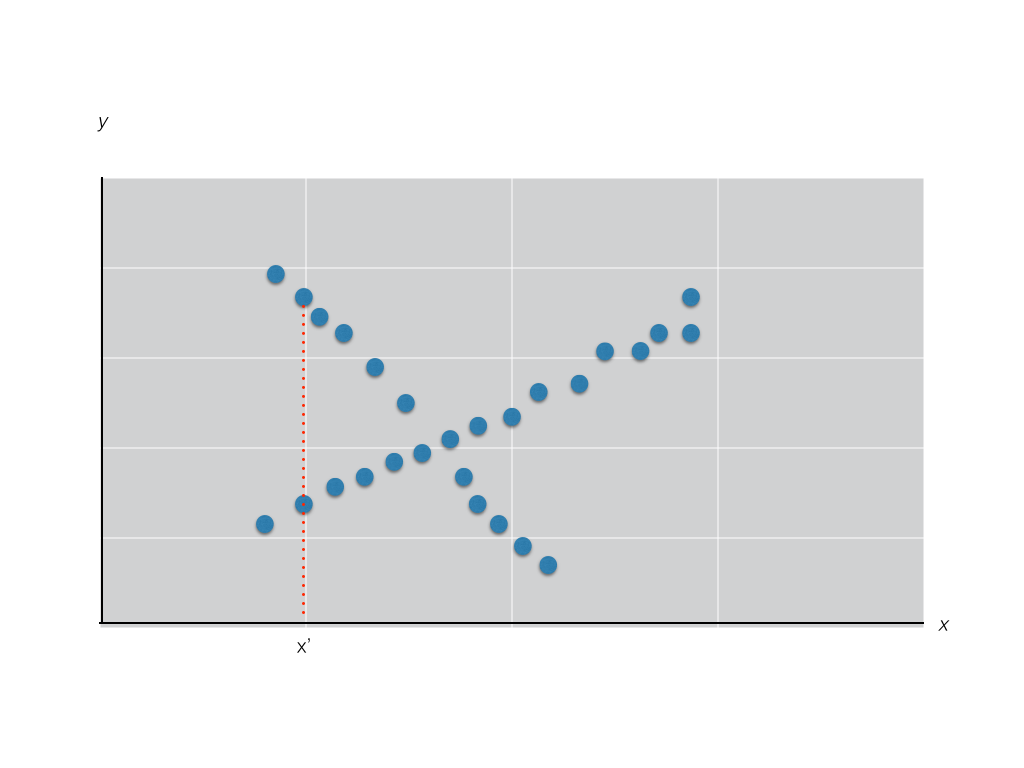
\includegraphics[width=0.4\textwidth,height=4cm]{drawings_007.png}   
 \label{fig:x-y}	}
\centering
\subfigure[Y $\mid$ X shoes single group in 2-D space, a single value is outpted
from averaging all the values in prediction set.]{
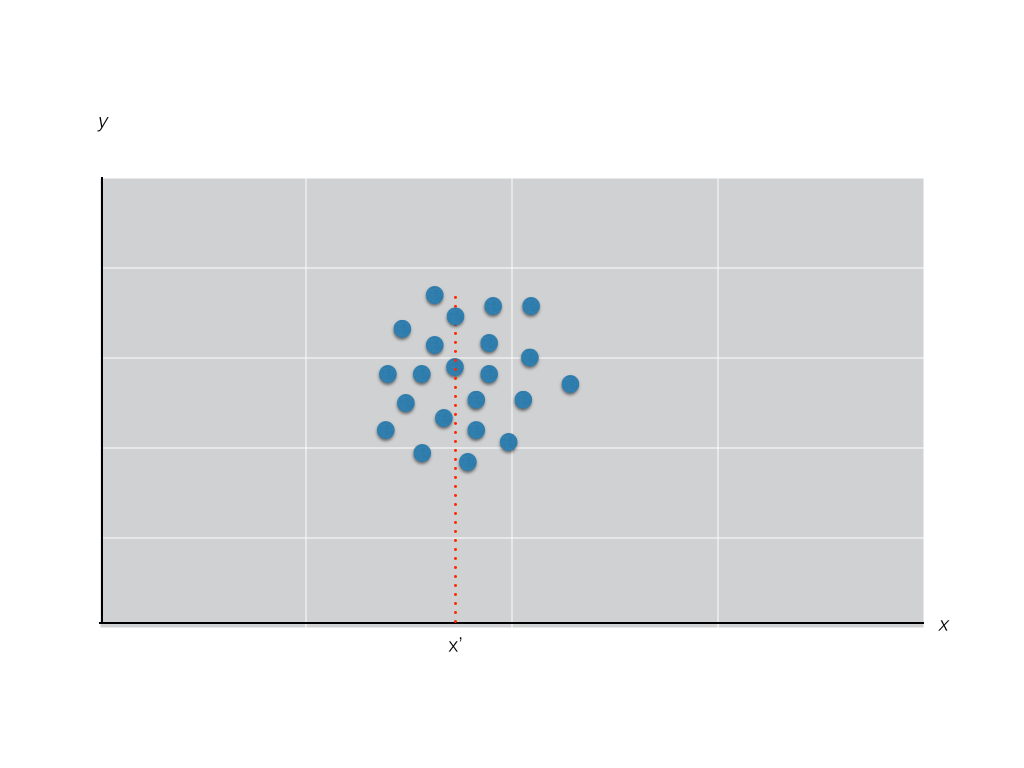
\includegraphics[width=0.4\textwidth,height=4cm]{drawings_008.png}   
 \label{fig:x-y}	}
\caption[Optional caption for list of figures]{Similarity Groups in 2-D plane
 }
\label{fig:subfigureExample}
\end{figure}
\subsubsection{A suitable measure for predictability}
A suitable measure for predictability \emph{Entropy} is used	
using probability of each 2-D class in the prediction values group(neighbors)	
Or a proportion test testing differences in the proportions using chi-squared
or z-test.(according to our model)
Given a prediction set of x' comprised of most similar x and his  neighbors in the prediction graph.
\begin{align*}
 x_s \cup N_s = \cup_{i=1}^{d2} \mathcal{N}_s^i
\end{align*}
 \begin{equation}
\mathcal{N}_{s}^{i} = \{ v \in \mathcal{N}_s \mid M_{2D}(v,y) =d_i  , i \in \{1\dots d2 \}\}
 \end{equation}
prediction group is now splitted according to their similarity in 2-D space.
  \begin{equation}
  p(d_i)=\dfrac{\mid \mathcal{N}_{s}^{i}\mid }{ \mid  N_s\mid }
  \end{equation}


\begin{enumerate}
 \item Calculate Entropy in 2D space.\\
   Without a loss of generality, let  $d_1, \dots ,d_{d2}$
   be ordered 2D Groups by probability $p(d2)$.
  \begin{equation}
 p(d_1)\leq p(d_2)\leq \dots \leq p(d_{d2})
  \end{equation}
  \begin{equation}
  Entropy^{2D} \equiv  \sum\limits_{i=1}^{d2} p(d_i) \times  log\dfrac{1}{p(d_i)}
  \end{equation}
  In order to standardize Entropy to the scale [0,1]\\
  Since entropy has the property:
    \begin{align*}
     H(x)= \sum\limits_{i=1}^{n} p(x) \times log\dfrac{1}{p(x)} \leq log_{2}n 
    \end{align*}
   
   We'll scale the entropy to [0,1]
  \begin{align*}
   Scaled\ Entropy^{2D} \equiv  \dfrac{Entropy^{2D}}{log_{2}d2}
  \end{align*}
  \item
  Another measure is by doing a proportions test
  checking to see if if there is no difference between two major groups.
  \begin{align*}
  H0: p(d1|x') -  p(d2|x') >0\\
  H1:p(d1|x') -  p(d2|x') \leq 0
  \end{align*}
  Assuming normality and parametric test we can
  simply give a thumb rule 
  \begin{align*} 
  p(d1|x') > 1.65 \times p(d1|x')\\
   \end{align*} 
   
   If the condition is met output single predictor
   otherwise output multiple  predictors.
\end{enumerate}




\subsection{Prediction Process}
Let 
$x' \in \mathbb{R}$  be  the predictor for which we want to find an estimator $\hat{y}$\\
Our prediction model is comprised of :
\begin{align*}
M_{1D} -\text{\emph{ mapping of x to similarity group in 1D}}
\end{align*}
\begin{align*}
M_{2D} -\text{\emph{ mapping of x to similarity group in 2D}}
\end{align*}
\begin{align*}
sim:X \times X \rightarrow \mathbb{R} - similarity\ fucntion.
\end{align*}
\begin{align*}
G_i(V_i,E_i) - prediction\ graphs
\end{align*}



\begin{enumerate}[(a)]

\item
  Find  similarity graph index
\begin{align*}
    s= M_{1D}( x^{'})
\end{align*}  
  \item
  Find most similar $v_s \in V_s$  to x' using the similarity function
  \begin{align*}
  v_s = v \in V_s \mid \ sim(x',v_j) \leq sim(x',v_s),\ \forall v_j \in V_s.
  \end{align*}
  $v_s$ is the vertex that links  the predictor x' $\in$ X (with unknown y), to 
  $G_s$ graph where each vertex has a corresponding y,
   thus linking a predictor in 1-D X to a graph in 2-D X-Y plane.
  \item
  Find $v_s$ neighbors from the  adjacency graph $G(V_s,E_s)$
\begin{align*}
    \mathcal{N}_s =  \lbrace  \  v_j  \mid \   (v_s,v_j)\in E_s\   \rbrace
\end{align*}  
 
  \item
  Group each $v_j\in \mathcal{N}_s$  $M_{2D}$
  to d2 similarity groups in 2D space.  
  \begin{align*}
  M_{2D}(v_j,y_j)\rightarrow d_j, \quad d_j\in\{1\dots d2\} 
  \end{align*}
  \item
  Split $\mathcal{N}_s$ according to 2D similarity groups:
   \begin{equation}
   \mathcal{N}_{s}^{1} ,\dots,\mathcal{N}_{s}^{d2}
 \end{equation}
  \begin{equation}
   \mathcal{N}_{s}^{i} = \{\  v \in N_s \  \mid \  M_{2D}(v) =d_i\   , i \in \{1\dots d2 \}\ \}
 \end{equation}
  \item Calculate probabilities of 2D  groups:\\
  \begin{equation}
  p(d_i)=\dfrac{\mid \mathcal{N}_{s}^{i}\mid }{ \mid  N_s\mid }
  \end{equation}
 
  \item
    Calculate estimators:   \\
    Average of outcome values of most similar x, $x_s=v_s$,  f($v_s$)=$y_s$\\and 
    and  its neighbors  in the graph for each 2D group:
    \begin{equation}     
  \hat y_i = \dfrac{f(v_s) + \sum\limits_{v \in \mathcal{N}_s^{i}} f(v)}{\vert \mathcal{N}_s^{i} \vert +1},\quad \forall i \in \{1\dots d2 \}
\label{eqn:simple_one} 
\end{equation}
\item Check predictability in 2D space and output estimator/s.\\
If $Scaled \ Entropy^{2D} < 0.4 \quad or\quad p(d_1\mid x') > 2\times p(d_2\mid x')$
output scalar\\
\begin{equation}
  \hat y = \hat{y}_1
\end{equation}
otherwise, output multiple outcomes vector:\\
\begin{equation}
  \hat y = (\hat{y}_1,\dots,\hat{y}_{d2})
\end{equation}
\end{enumerate}

\begin{figure}[ht]
\centering
\subfigure{
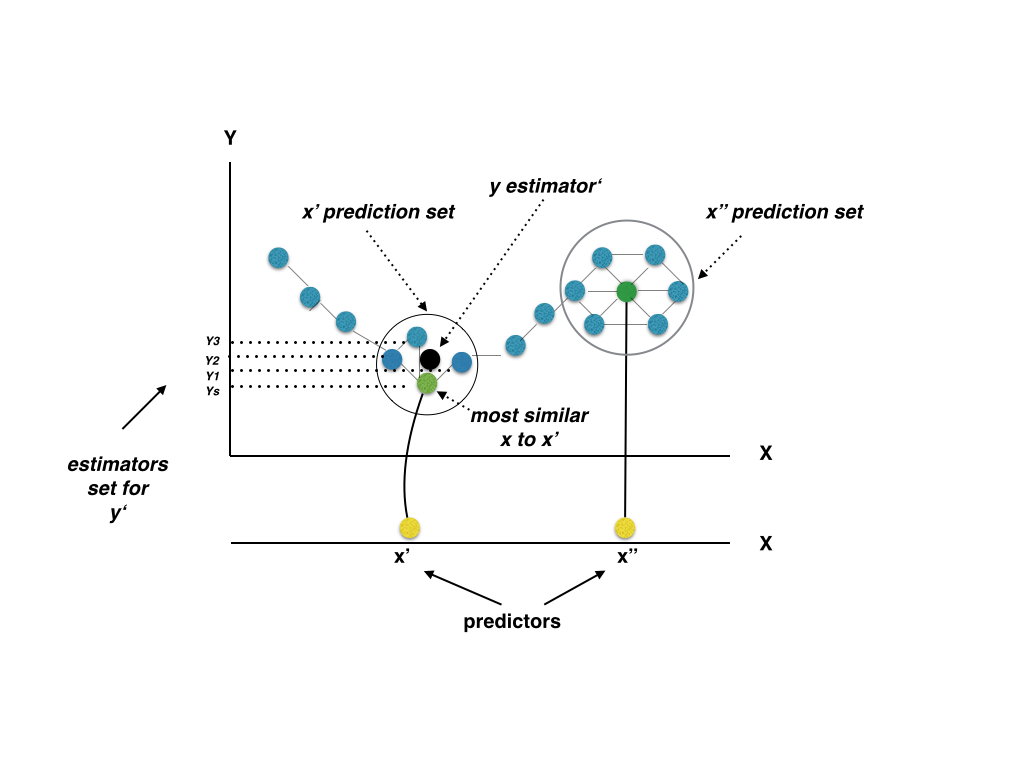
\includegraphics[width=0.7\textwidth,height=6cm]{drawings_010.png}   
 \label{fig:x-y}	}
\caption[Optional caption for list of figures]{Linking 1D(X) predictors to 2D (X-Y) Prediction Graph
 }
\label{fig:subfigureExample}
\end{figure}

 \begin{figure}[ht]
\centering
\subfigure{
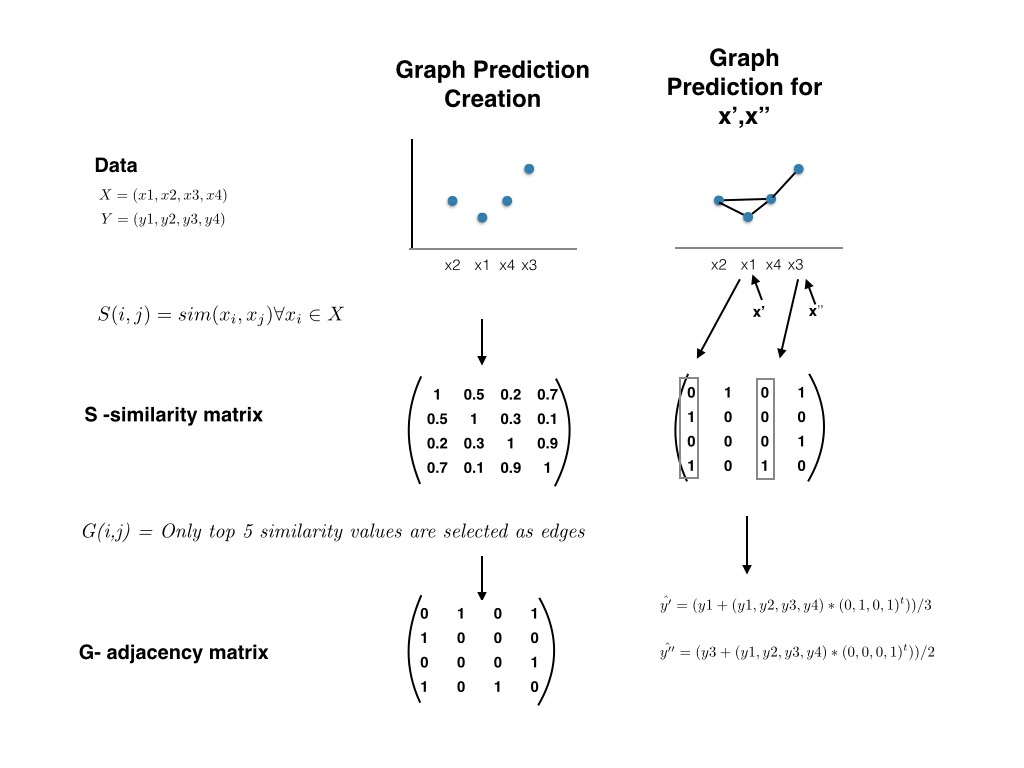
\includegraphics[width=0.7\textwidth,height=6cm]{drawings_009.png}   
 \label{fig:x-y}	}
\caption[Optional caption for list of figures]{Graph Creation And Prediction
 }
\label{fig:subfigureExample}
\end{figure}
\subsection{Graph Prediction As a Latent Graph Variable}
Besides being a a prediction model, graph prediction can be viewed as additional hidden graph information.
As such we can use the outcome of the graph model as a regressor 
in another model.
so if 
\begin{equation}
\hat{y}=\hat{y_{graph}}
\end{equation} a graph prediction,
a linear regression with one variable and latent graph variable will look:

\begin{equation}
\hat {y_{linear}}= ax+b+\hat {y_{graph}}
\end{equation}
$ \hat{y_{graph}}$ is simply graph prediction value(and a predictor of it's own right).
The choice of the model can be a model chosen from known models
which yields best performance.

\subsection{Generalization To Multidimensional Space}
the model was limited predictors in 1-D space. when $x\in \mathbb{R}^n$ we can handle in two a approaches
\begin{itemize}
\item  Similarity functions from $\mathbb{R}^n\rightarrow\mathbb{R}$
\item  A  function that pre process the data from $\mathbb{R}^n$ to $\mathbb{R} $
\end{itemize}
\subsection{KiNN Algorithm Pseudo Code}
%\begin{algorithm} [1]                
%\caption{KiNN Algorithm}          % give the algorithm a caption
%\label{alg1}                           % and a label for \ref{} commands later in the document
\underline{\textbf{\emph{Initialization}}}
\begin{algorithmic}
\small
\State$X=\{x_i, i=1\dots n \}$ the regressor group
\State $ Y=\{y_i\} $ the outcome group such that  $y_i = f(x_i)$ $\forall  i=1\dots n $.
\State $M_{1D}(x_i)=z_i, z_i \in \{1..d\}$ a mapping of predictor $x_i$ to similarity group $z_i$.
\State $M_{2D}(x_i,y_i)=z2_i, z2_i \in \{1..d2\}$ a mapping of pair ( $x_i,y_i)$ to similarity group $z2_i$.
\State $TopK(K,S)$ -Top K values in matrix $S_i$.
\end{algorithmic}
\underline{\textbf{\emph{Definitions}}}
\begin{algorithmic}
\small
\State $X_i$=Similarity groups.
\State $S_i$=Similarity matrices
\State $G_i(X_i,E_i)$=Adjacency  matrices
\end{algorithmic}
\underline{\textbf{\emph{Graph Creation}}}
\begin{algorithmic}
\small
\State $\{ X_i\}\leftarrow M_{1D}(X)$ \Comment{Map X into distinct  similarity groups }\\
\ForAll{ $X_i $} \Comment{Create similarity matrix for each similarity group}
\ForAll{ $ x_j,x_k\in X_i $} 
\State $S_i(j,k)\leftarrow similarity(x_j,x_k)$
\EndFor
\EndFor\\
\ForAll{ $S_i $}  \Comment{Eliminate self similarity in similarity matrices}
\State $S_i\leftarrow S_i- I$
\EndFor
\\
\ForAll{ $X_i $} \Comment{Calculate number of edges for each similarity group}

\State $\mid E_i \mid= MAX(({\mid X_i \mid}^{2}-\mid X_i \mid ) \times (1 -Corr(X_i,Y_i)^2),2\times \mid X_i \mid)$
\EndFor
\\
\ForAll{ $S_i $} \Comment{Create adjacency matrix from similarity matrix}
\ForAll{ $s_{j,k} \in S_i$} 
\If {$s_{j,k}\not\in TopK(S_i,\mid E_i \mid)$}
\State $g_{j,k} \leftarrow 0$
\Else
\State $g_{j,k} \leftarrow 1$
\EndIf
\EndFor
\EndFor
\end{algorithmic}
\underline{\textbf{\emph{Prediction}}}
\begin{algorithmic}
\small
\State $\boldsymbol {  X_s \leftarrow M_{1D}(x')}$\Comment{apply 1D model to the regressor to find a single similarity group}\\

\State  $\boldsymbol {x_s\leftarrow max(similarity(x',X_s))}$\Comment{find most similar value in similarity group }\\


\State $\boldsymbol {\mathcal{N}_s\leftarrow$  neighbors of $ x_s $ in graph $G_s}$\Comment{Find prediction group using most similar $x_s$ value in graph matrix}\\


\State $\boldsymbol {\hat y = \dfrac{f(x_s) + \sum\limits_{x_n \in \mathcal{N}_s} f(x_n)}
{\vert \mathcal{N}_s \vert +1}} $\Comment{Calculate estimator $\hat{y}$ by averaging predictor group $x_s$ and $\mathcal{N}_s$}\\
 \end{algorithmic}
%\end{algorithm}
\pagebreak


\newpage 
\section{Experiments}
In order to test the model performance we simulated several datasets
and compared performance to known models.
also includes test case with real movies dataset.
\subsection{Toy Examples}




\subsubsection{Dataset I}
%I
\begin{figure}[ht]
\centering
\subfigure[dataset points graph]{
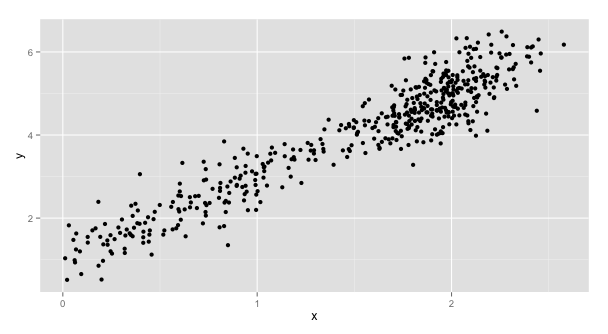
\includegraphics[width=0.4\textwidth]{I0}
   
    \label{fig:subfig1}	}
\subfigure[distribution patterns]{

    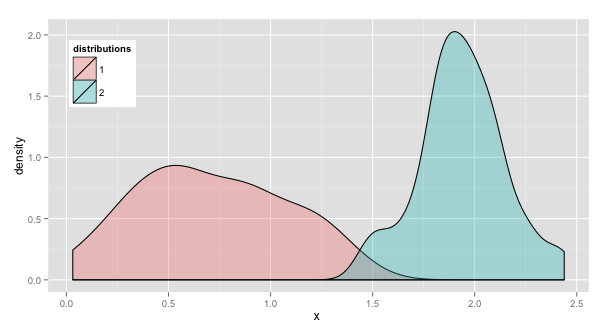
\includegraphics[width=0.4\textwidth]{I0d}
    \label{fig:subfig2}
}
\subfigure[similarity graphs]{
    \includegraphics[width=0.4\textwidth]{I0g}
    \label{fig:subfig3}
}
\subfigure[models predictions]{
  %  \rule{4cm}{3cm}
  \includegraphics[width=0.4\textwidth]{I0t}
    \label{fig:subfig4}
}
\caption[Optional caption for list of figures]{\subref{fig:subfig1} Dataset I points plot , \subref{fig:subfig2} Mixture Models distributions patterns found using EM \subref{fig:subfig3}similarity graph created for each pattern
\subref{fig:subfig4} models and y.
\\
All models capture the same accuracy the linearity of the dataset, regression tree was less accurate due to his step like nature. }
\label{fig:subfigureExample}

\end{figure}




%II
\subsubsection{Dataset II}
\begin{figure}[H]
\centering
\subfigure[dataset points graph]{
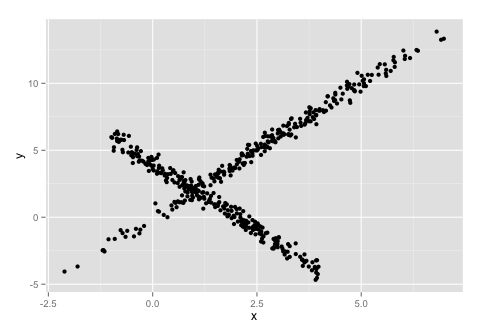
\includegraphics[width=0.4\textwidth]{II0}
 \label{fig:subfig1}	
 }
 \centering
\subfigure[distribution patterns]{
    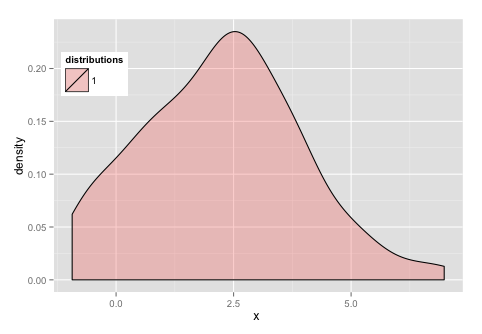
\includegraphics[width=0.4\textwidth]{IId}
    \label{fig:subfig2}
}

\subfigure[similarity graphs]{
    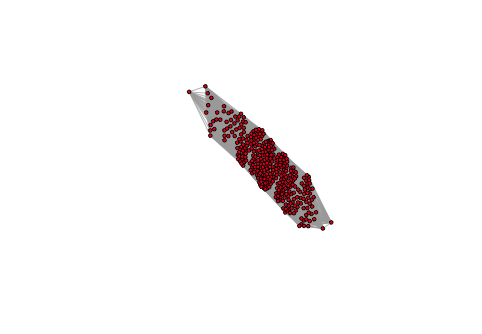
\includegraphics[width=0.6\textwidth]{pIIg}
    \label{fig:subfig3}
}

\subfigure[similarity graphs]{
    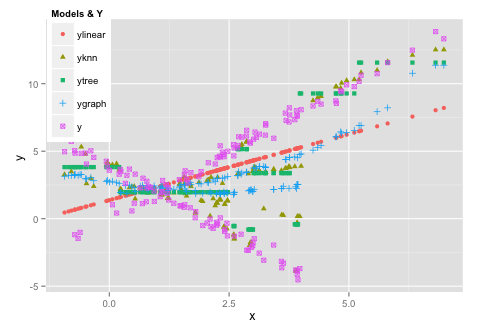
\includegraphics[width=0.4\textwidth]{pIIt2}
    \label{fig:subfig5}
}



\caption[Optional caption for list of figures]{
\subref{fig:subfig1} Dataset II points form an X like pattern.
\subref{fig:subfig2}only one distribution found
\subref{fig:subfig3} single graph formed for the density pattern
\subref{fig:subfig4} prediction in lines plot and y dashed.
\subref{fig:subfig5} prediction points and y
Linear model does not well with two opposite slopes, k-NN and CART about the same.
in graph model layer one similarity density failed, and we are left with single graph.  After removing edges (k edges density parameter) the graph model surpass other models by at least 10\%.
}
 \label{fig:subfigureExample}

\end{figure}

%IV
\subsubsection{Dataset III}
\begin{figure}[H]
\centering
\subfigure[dataset points plot]{
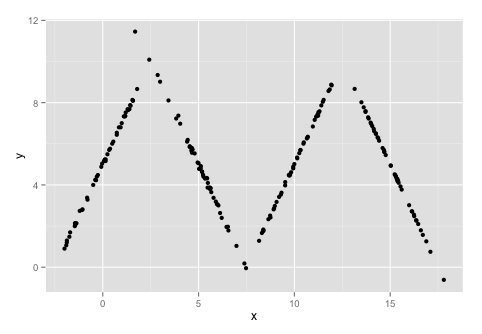
\includegraphics[width=0.4\textwidth]{III0}
   \label{fig:subfig1}	}
\subfigure[distribution patterns]{

    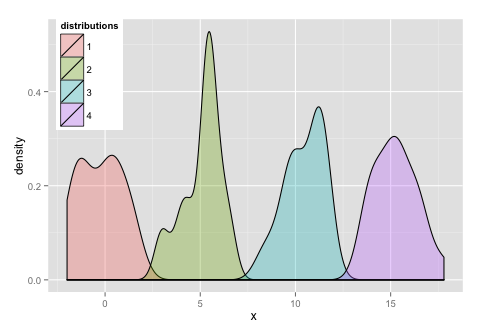
\includegraphics[width=0.4\textwidth]{IIId}
    \label{fig:subfig2}
}
\subfigure[similarity graphs]{
    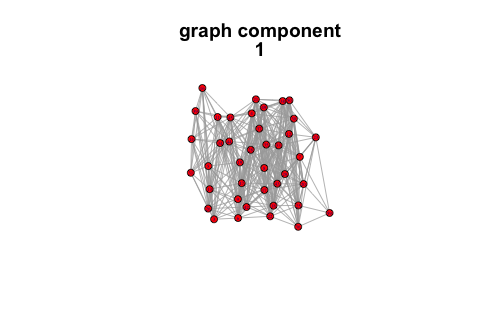
\includegraphics[width=0.4\textwidth]{pIII1}
    \label{fig:subfig3}
}
\subfigure[similarity graphs]{
    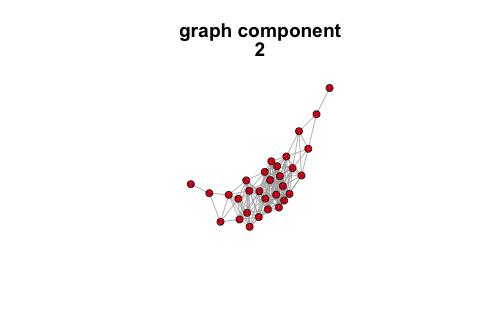
\includegraphics[width=0.4\textwidth]{pIII2}
    \label{fig:subfig4}
}
\subfigure[similarity graphs]{
    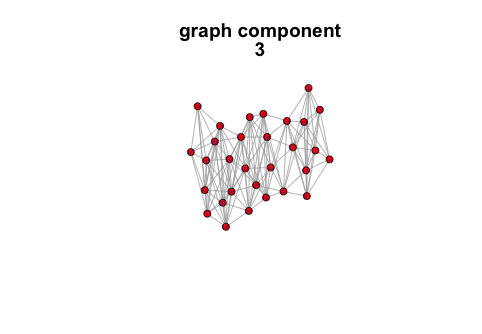
\includegraphics[width=0.4\textwidth]{pIII3}
    \label{fig:subfig5}
}
\subfigure[similarity graphs]{
    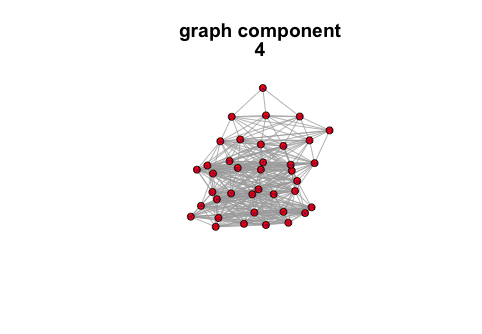
\includegraphics[width=0.4\textwidth]{pIII4}
    \label{fig:subfig6}
}
\subfigure[models predictions lines]{
  %  \rule{4cm}{3cm}
  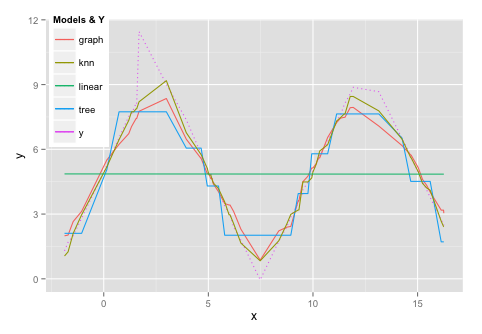
\includegraphics[width=0.4\textwidth]{pIIIt1}
    \label{fig:subfig7}
}
\subfigure[models predictions-points]{
  %  \rule{4cm}{3cm}
  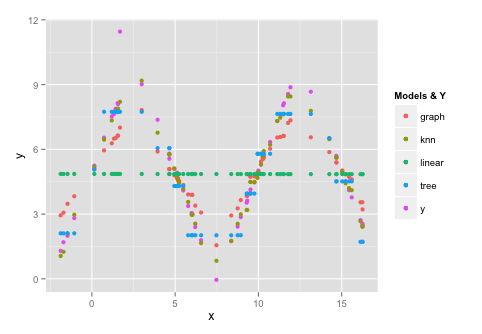
\includegraphics[width=0.4\textwidth]{pIIIt2}
    \label{fig:subfig8}
}
\caption[Optional caption for list of figures]{
Linear model prediction fails due to opposite linear slopes. CART 
and k-NN uses locality well, in graph we need to pick less denser graph(less edges) to minimize effect of distant neighbors.CART models does less well due to more averaging nature.(as in Dataset I )}
\label{fig:subfigureExample}
\end{figure}

%IV
\subsubsection{Dataset IV}
\begin{figure}[H]

\centering
\subfigure[dataset points graph]{
\includegraphics[width=0.4\textwidth]{IV0}
   
    \label{fig:subfig1}	}
\subfigure[distribution patterns]{

    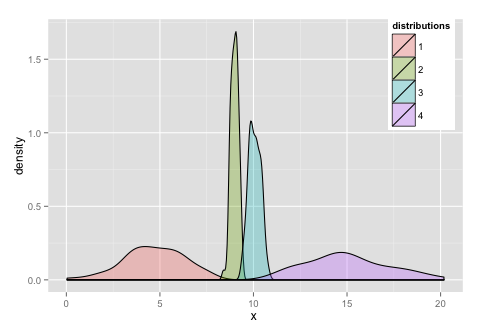
\includegraphics[width=0.4\textwidth]{IVd}
    \label{fig:subfig2}
}
\subfigure[similarity graphs]{
    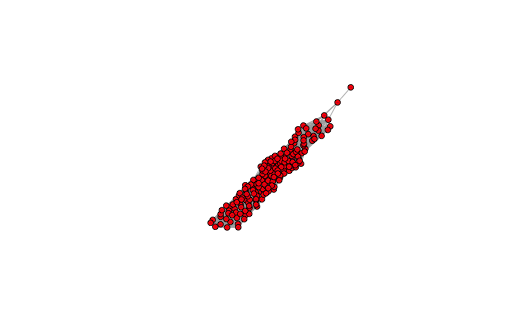
\includegraphics[width=0.4\textwidth]{pIV1}
    \label{fig:subfig3}
}
\subfigure[similarity graphs]{
    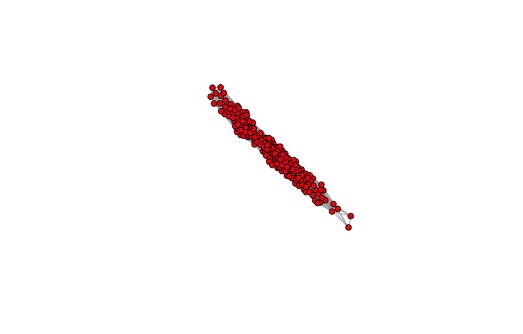
\includegraphics[width=0.4\textwidth]{pIV2}
    \label{fig:subfig3}
}
\subfigure[similarity graphs]{
    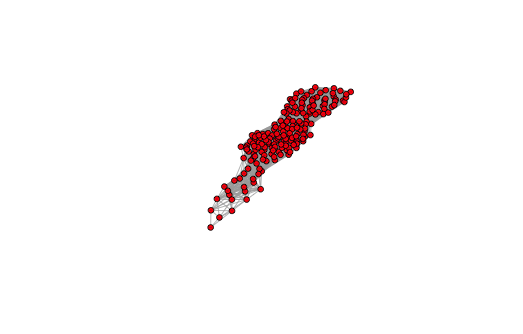
\includegraphics[width=0.4\textwidth]{pIV3}
    \label{fig:subfig4}
}
\subfigure[similarity graphs]{
    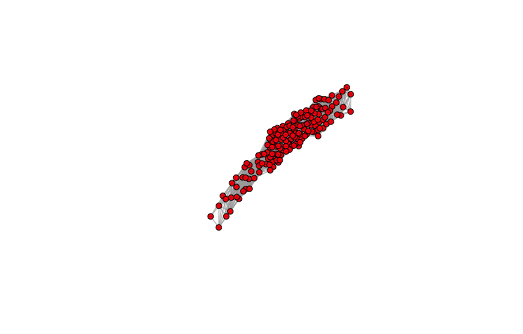
\includegraphics[width=0.4\textwidth]{pIV4}
    \label{fig:subfig5}
}
\subfigure[models predictions]{
  %  \rule{4cm}{3cm}
  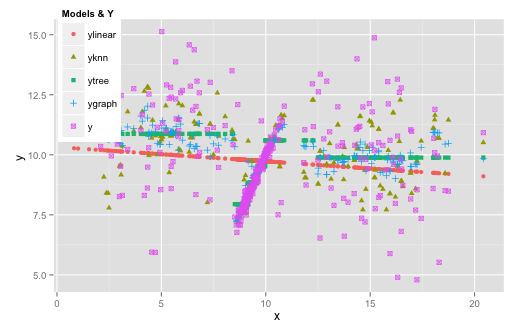
\includegraphics[width=0.4\textwidth]{pIVt}
    \label{fig:subfig6}
}
\caption[Optional caption for list of figures]{
Linear model fails in the presence of linear line within of two noise patterns.
Graph and k-NN capture the same accuracy the linearity of the dataset, the regression tree-while we can assume that it does as well as k-NN and graph models in prediction of the noise, the linear part subjected to to much averaging. }



\label{fig:subfigureExample}

\end{figure}


%VE
 \subsubsection{Dataset V}
\begin{figure}[H]
\centering
\subfigure[dataset points graph]{
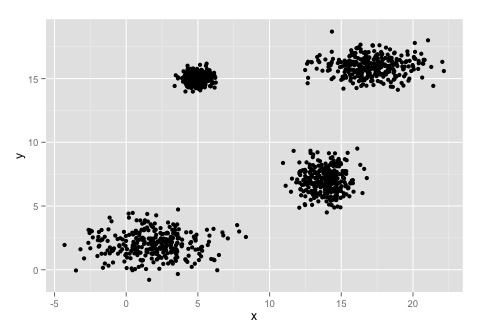
\includegraphics[width=0.4\textwidth]{VE0}
   
    \label{fig:subfig1}	}
\subfigure[distribution patterns]{

    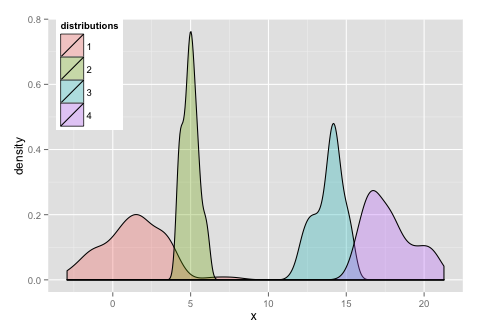
\includegraphics[width=0.4\textwidth]{VEd}
    \label{fig:subfig2}
}
\subfigure[similarity graphs]{
    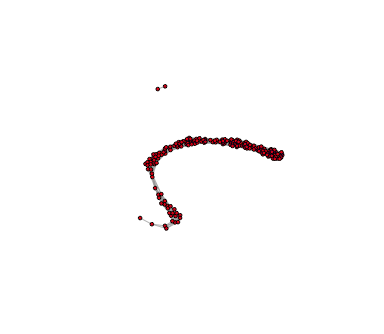
\includegraphics[height=4cm,width=0.4\textwidth]{VEg1}
    \label{fig:subfig3}
}
\subfigure[similarity graphs]{
    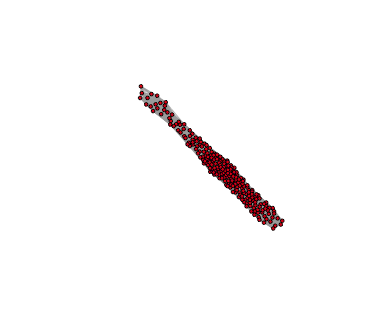
\includegraphics[height=4cm,width=0.4\textwidth]{VEg2}
    \label{fig:subfig4}
}
\subfigure[similarity graphs]{
    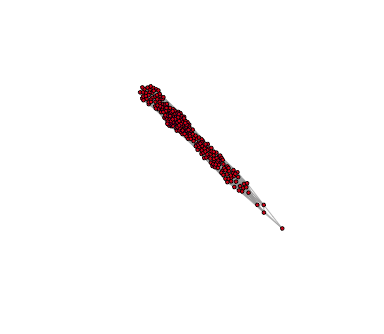
\includegraphics[height=4cm,width=0.4\textwidth]{VEg3}
    \label{fig:subfig5}
}
\subfigure[similarity graphs]{
    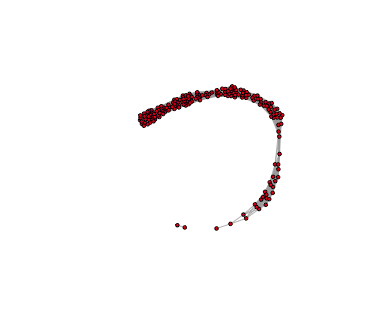
\includegraphics[height=4cm,width=0.4\textwidth]{VEg4}
    \label{fig:subfig6}
}

\subfigure[models predictions]{
  %  \rule{4cm}{3cm}
  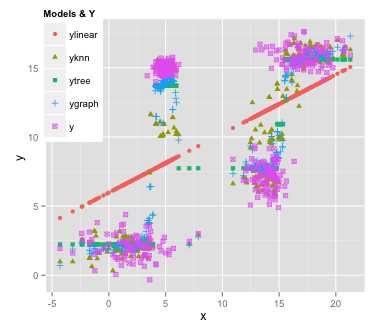
\includegraphics[height=4cm ,width=0.4\textwidth]{VEt2}
    \label{fig:subfig8}
}
\caption[Optional caption for list of figures]{

Linear model fails in presence of noise. CART and graph manage to predict better then when some pattern emerges(different distributions mean and sd,points can be splitted to rectangles by CART).
differences are negligible.
k-NN does less well locality of x does not distinguish well between groups/patterns. }
\label{fig:subfigureExample}

\end{figure}

\subsubsection{Results summary}
\begin{table}[ht!]
\centering
\caption{Models Performance-  R squared results }

\begin{tabular}{c c c c c}

\hline 
\hline

Dataset & Linear Regression & CART  & KNN & •Graph Model\\ 
\hline 
I &100 & 94 & 99 & 100\\ 

II &14  & 35 &35&45 \\ 

 III &0 & 90 & 99 & 99 \\ 

 IV  & 0 & 25 & 33&36 \\ 

V  &24 &60 & 72 & 72 \\ 

\hline 
\end{tabular} 
\end{table}
\subsection{Case Study-Predicting Movies Revenues}

In this case study we would like apply our model to predict future movies revenues.
Here are sample records from the movies dataset:\\

\renewcommand{\arraystretch}{1.2}
\begin{tabular}{c c c c | c}

Genre& Director&Name&Budget&Revenue\\
\hline
Romantic&A.Hiller&Love Story&1M\$&10M\$\\
SciFi&J,Cameron & Terminator &1M\$&100M\$\\
Action&S,Stalone&Rocky 3&1M\$&50M\$\\
\hline
\end{tabular}
\paragraph{Pre Processing And Metric}
In applying graph methods we encounter a metric problems .
How to measure similarity when categorical variables are involved(how similar  is  sci-fi Genre to Romantic and how to weight it in the model)
In how to compute graph model prediction in more than one dimension?
scaling in the dataset preset another problem.
As the numeric values may vary significantly.
In order to handle the metric problems
we tie the regressors to the independent variable (revenue) by a linear regression.
so the linear regression output $\hat{y_reg}$ serves as an input for our graph model, thus achieving:
\begin{itemize}
\item dimensionality reduction, all regressors
are distilled into one regressor for the graph model
$x_{graph}=\hat{y_{reg}}$
\item
 solve weights problems for categorical variables through linear regression
\end{itemize}
To deal with independent and dependent variable range
use log scale.\\
In a sense we piggybacking linear regression model 
results in order to get better predictions in our graph model.\\
We also made a second graph model Called \textbf{Linear Graph Model}, now the results of the graph model are fed to a linear regression model as an extra latent variable containing graph information.

\subsubsection{Prediction}

%movies dataset
\begin{figure}[H]
\centering
\subfigure[movies dataset points]{
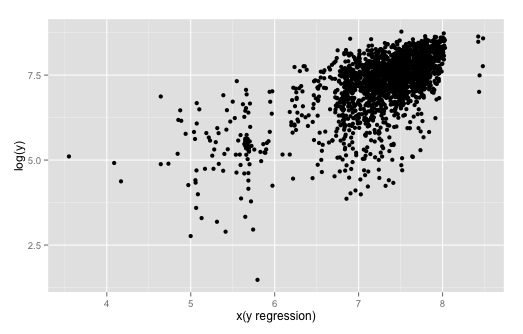
\includegraphics[width=0.4\textwidth]{M0} 
 \label{fig:subfig1}	}
\subfigure[movies distribution patterns]{

    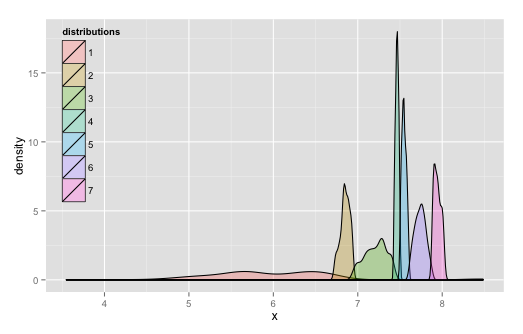
\includegraphics[width=0.4\textwidth]{M3}
    \label{fig:subfig2}
}
\subfigure[graph component  1]{
    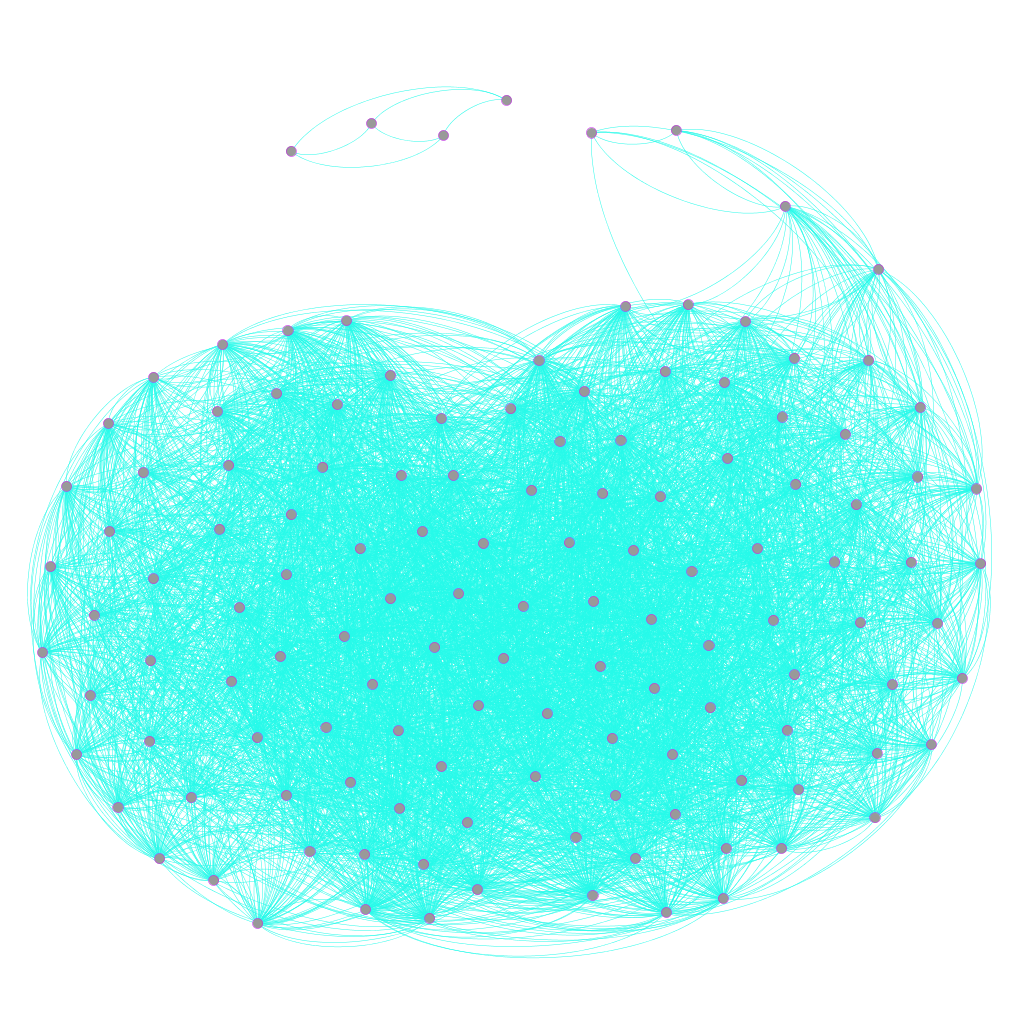
\includegraphics[width=0.4\textwidth,height=4cm]{g1}
    \label{fig:subfig3}
}
\subfigure[graph component  2]{
    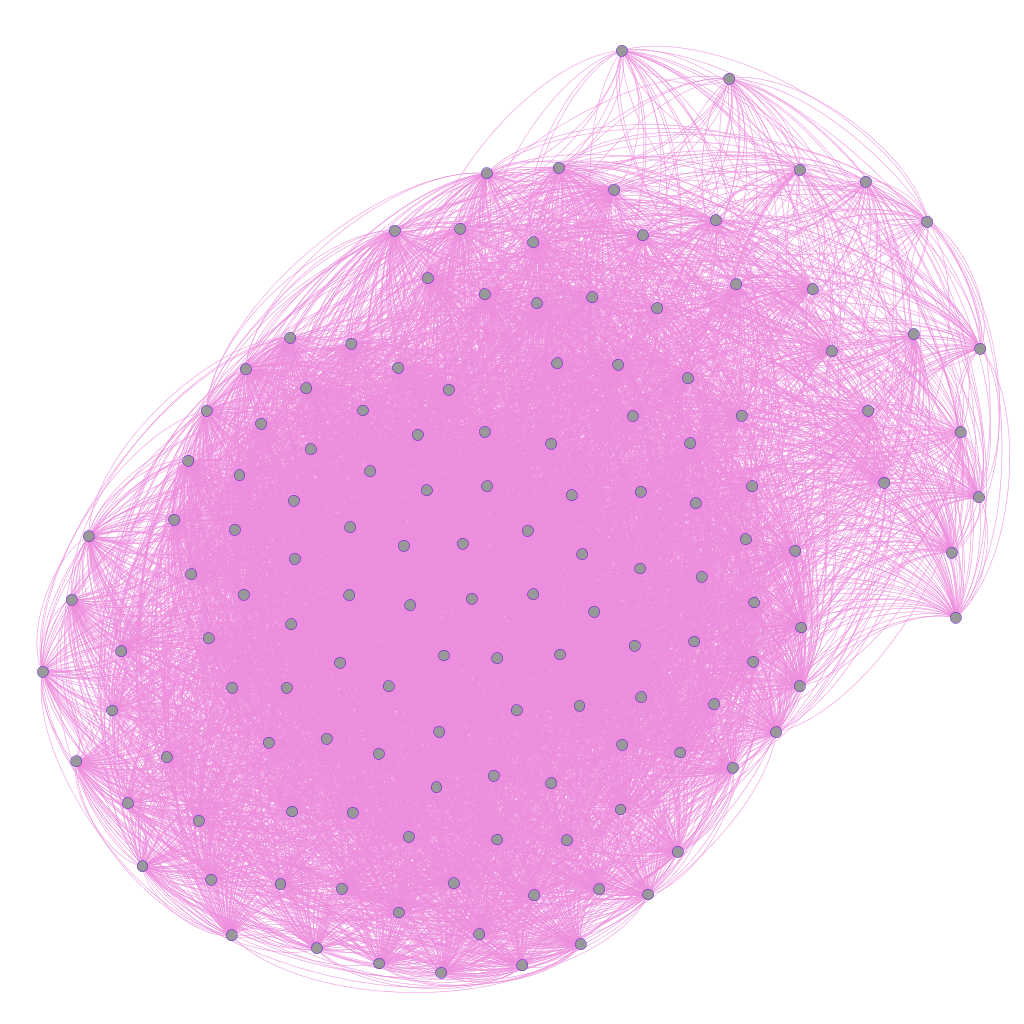
\includegraphics[width=0.4\textwidth,height=4cm]{g2}
    \label{fig:subfig3}
}
\subfigure[movies similarity density points]{
    \includegraphics[width=0.4\textwidth]{M1}
    \label{fig:subfig5}
}
\subfigure[models predictions and y (log revenues)]{
    \includegraphics[width=0.4\textwidth]{M4}
    \label{fig:subfig6}
}


\caption[Optional caption for list of figures]{
\subref{fig:subfig1} movies Dataset points plot using single variable x which is the output
linear regression.

Linear model does  find a linear connection. 
graph model is doing around more than 10% better.
when plugging graph model as another predictor we mange to
to increase prediction accuracy by 20\%.

}
\label{fig:subfigureExample}

\end{figure}

\subsubsection{Results Summary}
\begin{table}[ht!]
\centering
\caption{Models Performance-  R squared results }

\begin{tabular}{c c c c}

\hline 
\hline
Dataset&Linear Regression & Graph Model  & Linear-Graph Regression\\ 
\hline 
Log(Revenue) &41 & 53 & 60\\ 

Revenue   &22  & 34 &40 \\ 
\hline 
\end{tabular} 
\end{table}


\section{Conclusion}
In the experiments we saw that using finding hidden pattern followed by  creating similarity matrices  enabled us to create graph representation of
otherwise flat dataset.
which  can be fine-tuned - made dense or sparse according to edge density parameter \emph{K}

Application of the model  the simulated various datasets the model  managed to perform \emph{at least as good} as the best performing model.

In the movies dataset we took results of regression and the "real"  independent values
and extracted the graph model.
 Using graph model and regression results as two predictors in a new linear model:\\
$\hat{y}  = \hat{y}_{reg} + \hat{y}_{graph} + \epsilon$\\
which performed even better than both linear and graph model by 10-20%.
The graph model framework is also flexible.
we can replace layer 1 density similarity (EM and Mixture model) by different model.
Another similarity function (the model used Gaussian kernel ) can be used
and \emph{K} which is similar to all graphs can be picked (or calculated automatically) according to each component parameters (linear groups for instance prefer less edges ) 
and $\hat{y}_{graph}$ can be used as a predictor representing graph feature in another  model. (like in movies dataset)




\section{Bibliography}
\begin{thebibliography}{9}

\bibitem{sochreg}
Hao Ma,Michael R. Lyu,Irwin King , Dengyong Zhou,Chao Liu
  \emph{Recommender Systems with Social Regularization}.
 Proceeding
WSDM '11 Proceedings of the fourth ACM international conference on Web search and data mining
Pages 287-296 
\bibitem{patsim}
    Sebastian Klenk, Ju ̈rgen Dippon, Peter Fritz, and Gunther Heidemann ,Stuttgart University
  \emph{Determining Patient Similarity in Medical Social Networks}
   Proc. the First International Workshop on Web Science and Information Exchange in the Medical Web (MedEx 2010).  Raleigh, USA,  2010, Accepted.
 
\bibitem{simrank}
    G. Jeh and J. Widom
  \emph{SimRank: A Measure of Structural-Context Similarity}
  Proceedings of the Eighth ACM SIGKDD International Conference on Knowledge Discovery and Data Mining, pages 538-543, Edmonton, Canada, July 2002.
\bibitem{graphlayers}
 Zan Huang, Wingyan Chung, Thian-Huat Ong, Hsinchun Chen 
\emph{A Graph-based Recommender System for Digital Library}
Artificial Intelligence Lab  ,Department of Management Information Systems 
The University of Arizona Tucson, Arizona

\bibitem{mining}
Deng Cai, Zheng Shao, Xiaofei He, Xifeng Yan ,Jiawei Han
\emph{Mining Hidden Community in Heterogeneous Social Networks}
Department of Computer Science, University of Illinois at Urbana-Champaign ‡ Department of Computer Science, University of Chicago
\bibitem{kernel}
Modeling Social Strength in Social Media Community via Kernel-based Learning
Jinfeng Zhuang, Tao Mei, Steven C. H. Hoi, Xian-Sheng Hua, Shipeng Li
\bibitem{em}
Dempster, A.P.; Laird, N.M.; Rubin, D.B. (1977). "Maximum Likelihood from Incomplete Data via the EM Algorithm". Journal of the Royal Statistical Society, Series B 39 (1): 1–38. JSTOR 2984875. MR 0501537.  
\bibitem{book1}
\emph{An Introduction to Statistical Learning}
Gareth James Daniela Witten Trevor Hastie Robert Tibshirani.

\bibitem{pagerank}
Brin, S.; Page, L. (1998). "The anatomy of a large-scale hypertextual Web search engine". Computer Networks and ISDN Systems 30: 107–117

\bibitem{er}
 Erd\H{o}s-R\'enyi, A. (1959). "On Random Graphs". Publicationes Mathematicae 6: 290–297.

 \bibitem{optics}
Mihael Ankerst, Markus M. Breunig, Hans-Peter Kriegel, Jörg Sander (1999). OPTICS: Ordering Points To Identify the Clustering Structure. ACM SIGMOD international conference on Management of data. ACM Press. pp. 49–60.
\end{thebibliography}



 \pagebreak

\end{document}
